%%% 2023年 1月30日 星期一 13时46分30秒 CST
%%% author: Shao-Dan Lee 李小丹 字 殊恒

%\documentclass[a4paper,twoside]{article}
\documentclass[a4paper,twoside]{memoir}

%%% 2022年 7月30日 星期六 10时49分17秒 CST
%%% author: 李小丹(Shao-Dan Lee) 字 殊恒(Shuheng)

\usepackage[utf8]{inputenc}
\usepackage{latexsym}
\usepackage{textcomp}
\usepackage[no-math]{fontspec}
\usepackage[defaultfam,tabular,lining,scaled=1.02]{montserrat}
\usepackage[varqu,varl]{zi4} % sans serif typewriter
% \usepackage[scaled=1.1]{newtxsf} %or stix2
% \usepackage[defaultmathsizes,italic]{mathastext}
\usepackage{expl3}
% \usepackage{makeidx}
% \usepackage{verbatim}
% \usepackage[runin]{abstract}
\usepackage[margin=2cm,hmarginratio=1:1]{geometry}
\usepackage{graphicx}
% \usepackage[svgnames,table]{xcolor}
\usepackage[svgnames]{xcolor}
\usepackage{tikz}
\usepackage{lilyglyphs}
\usepackage[most]{tcolorbox}
\usepackage{multicol}
% The package "background" is not good,
% may use tikz or eso-pic
% cf. https://tex.stackexchange.com/questions/167719/how-to-use-background-image-in-latex
\usepackage[some]{background}
\usepackage{soul}
%\usepackage{emoji}
\usepackage[fixed]{fontawesome5}
% \usepackage{byo-twemojis}
\usepackage{twemojis}
% \usepackage{ulem}
\usepackage{enumitem}
\usepackage{calc}
% \usepackage{ifthen}
% \usepackage[center]{titlesec}
\usepackage[calcwidth]{titlesec}
\usepackage{tocdata}
%\usepackage{tocloft}
\usepackage{fancyhdr}
\usepackage{multirow}
\usepackage{longtable}
\usepackage{tabu}
\usepackage{multirow}
\usepackage{pgfornament}
% \usepackage{qrcode}
%%% cf. https://github.com/EagleoutIce/fancyqr/
\usepackage{fancyqr}
\usepackage{changelog}
\usepackage{xeCJK}
\usepackage[fontset=macnew]{ctex}

\makeatletter


\newcommand{\mytitle}{乐谱集}
\newcommand{\myname}{Shao-Dan Lee}
\newcommand{\mycnname}{李小丹\ 编著}
\newcommand{\myemail}{leeshuheng@icloud.com}

\author{\mycnname}
\title{\mytitle}
%\email{\myemail}
\date{\today}

\usepackage[bookmarks, pdfpagelabels, colorlinks]{hyperref}

% \usepackage{amsrefs}
\usepackage{bookmark}
\usepackage[noabbrev]{cleveref}
% polyglossia package should be last loaded.
\usepackage{polyglossia}

\usetikzlibrary{graphs}
\usetikzlibrary{shapes.misc}
\usetikzlibrary {shapes.callouts}
\usetikzlibrary{shadows}
\usetikzlibrary{chains}
\usepgflibrary {shadings}

\hypersetup {
	pdftitle={\mytitle},
	pdfsubject={Music score},
	pdfauthor={李小丹},
	pdfcreator={李小丹},
	%citecolor = MediumVioletRed,
	% citecolor = DarkViolet,
	citecolor = BlueViolet,
	linkcolor = RoyalBlue,
	%urlcolor = SeaGreen
	urlcolor = DarkTurquoise
}

%% from %%%
%% https://tug.org/pipermail/xetex/2008-December/011420.html
% \newfontfamily\semibf{FiraSans SemiBold}
%% https://tex.stackexchange.com/questions/536367/how-do-i-use-light-normal-semibold-and-bold-font-types-in-one-document-using
% \newcommand{\mynotation}{\textbf{\sourcesansprolight\underline{Notation}}}
% \newcommand{\mynotation}{\firasemibold\underline{Notation}}
\newcommand{\mynotation}{\fontseries{semibold}\selectfont Notation}
% \newcommand{\mynotation}{\fontseries{semibold}\selectfont\underline{Notation}}

% \renewcommand{\thefootnote}{\fnsymbol{footnote}}
% \renewcommand{\thefootnote}{\alph{footnote}}

% \renewcommand{\cftsecleader}{\bfseries\cftdotfill{\cftdotsep}}
% \renewcommand{\cftsecleader}{\cftdotfill{\cftdotsep}}

% \ctexset{fontset = macnew}
%\lishu and \youyuan

\def\cclink{https://creativecommons.org/licenses/by/4.0/}
\def\ccby{\href{\cclink}{\faCreativeCommons\faCreativeCommonsBy}}

\backgroundsetup{
	scale=1,
	angle=0,
	opacity=1,
	contents={
		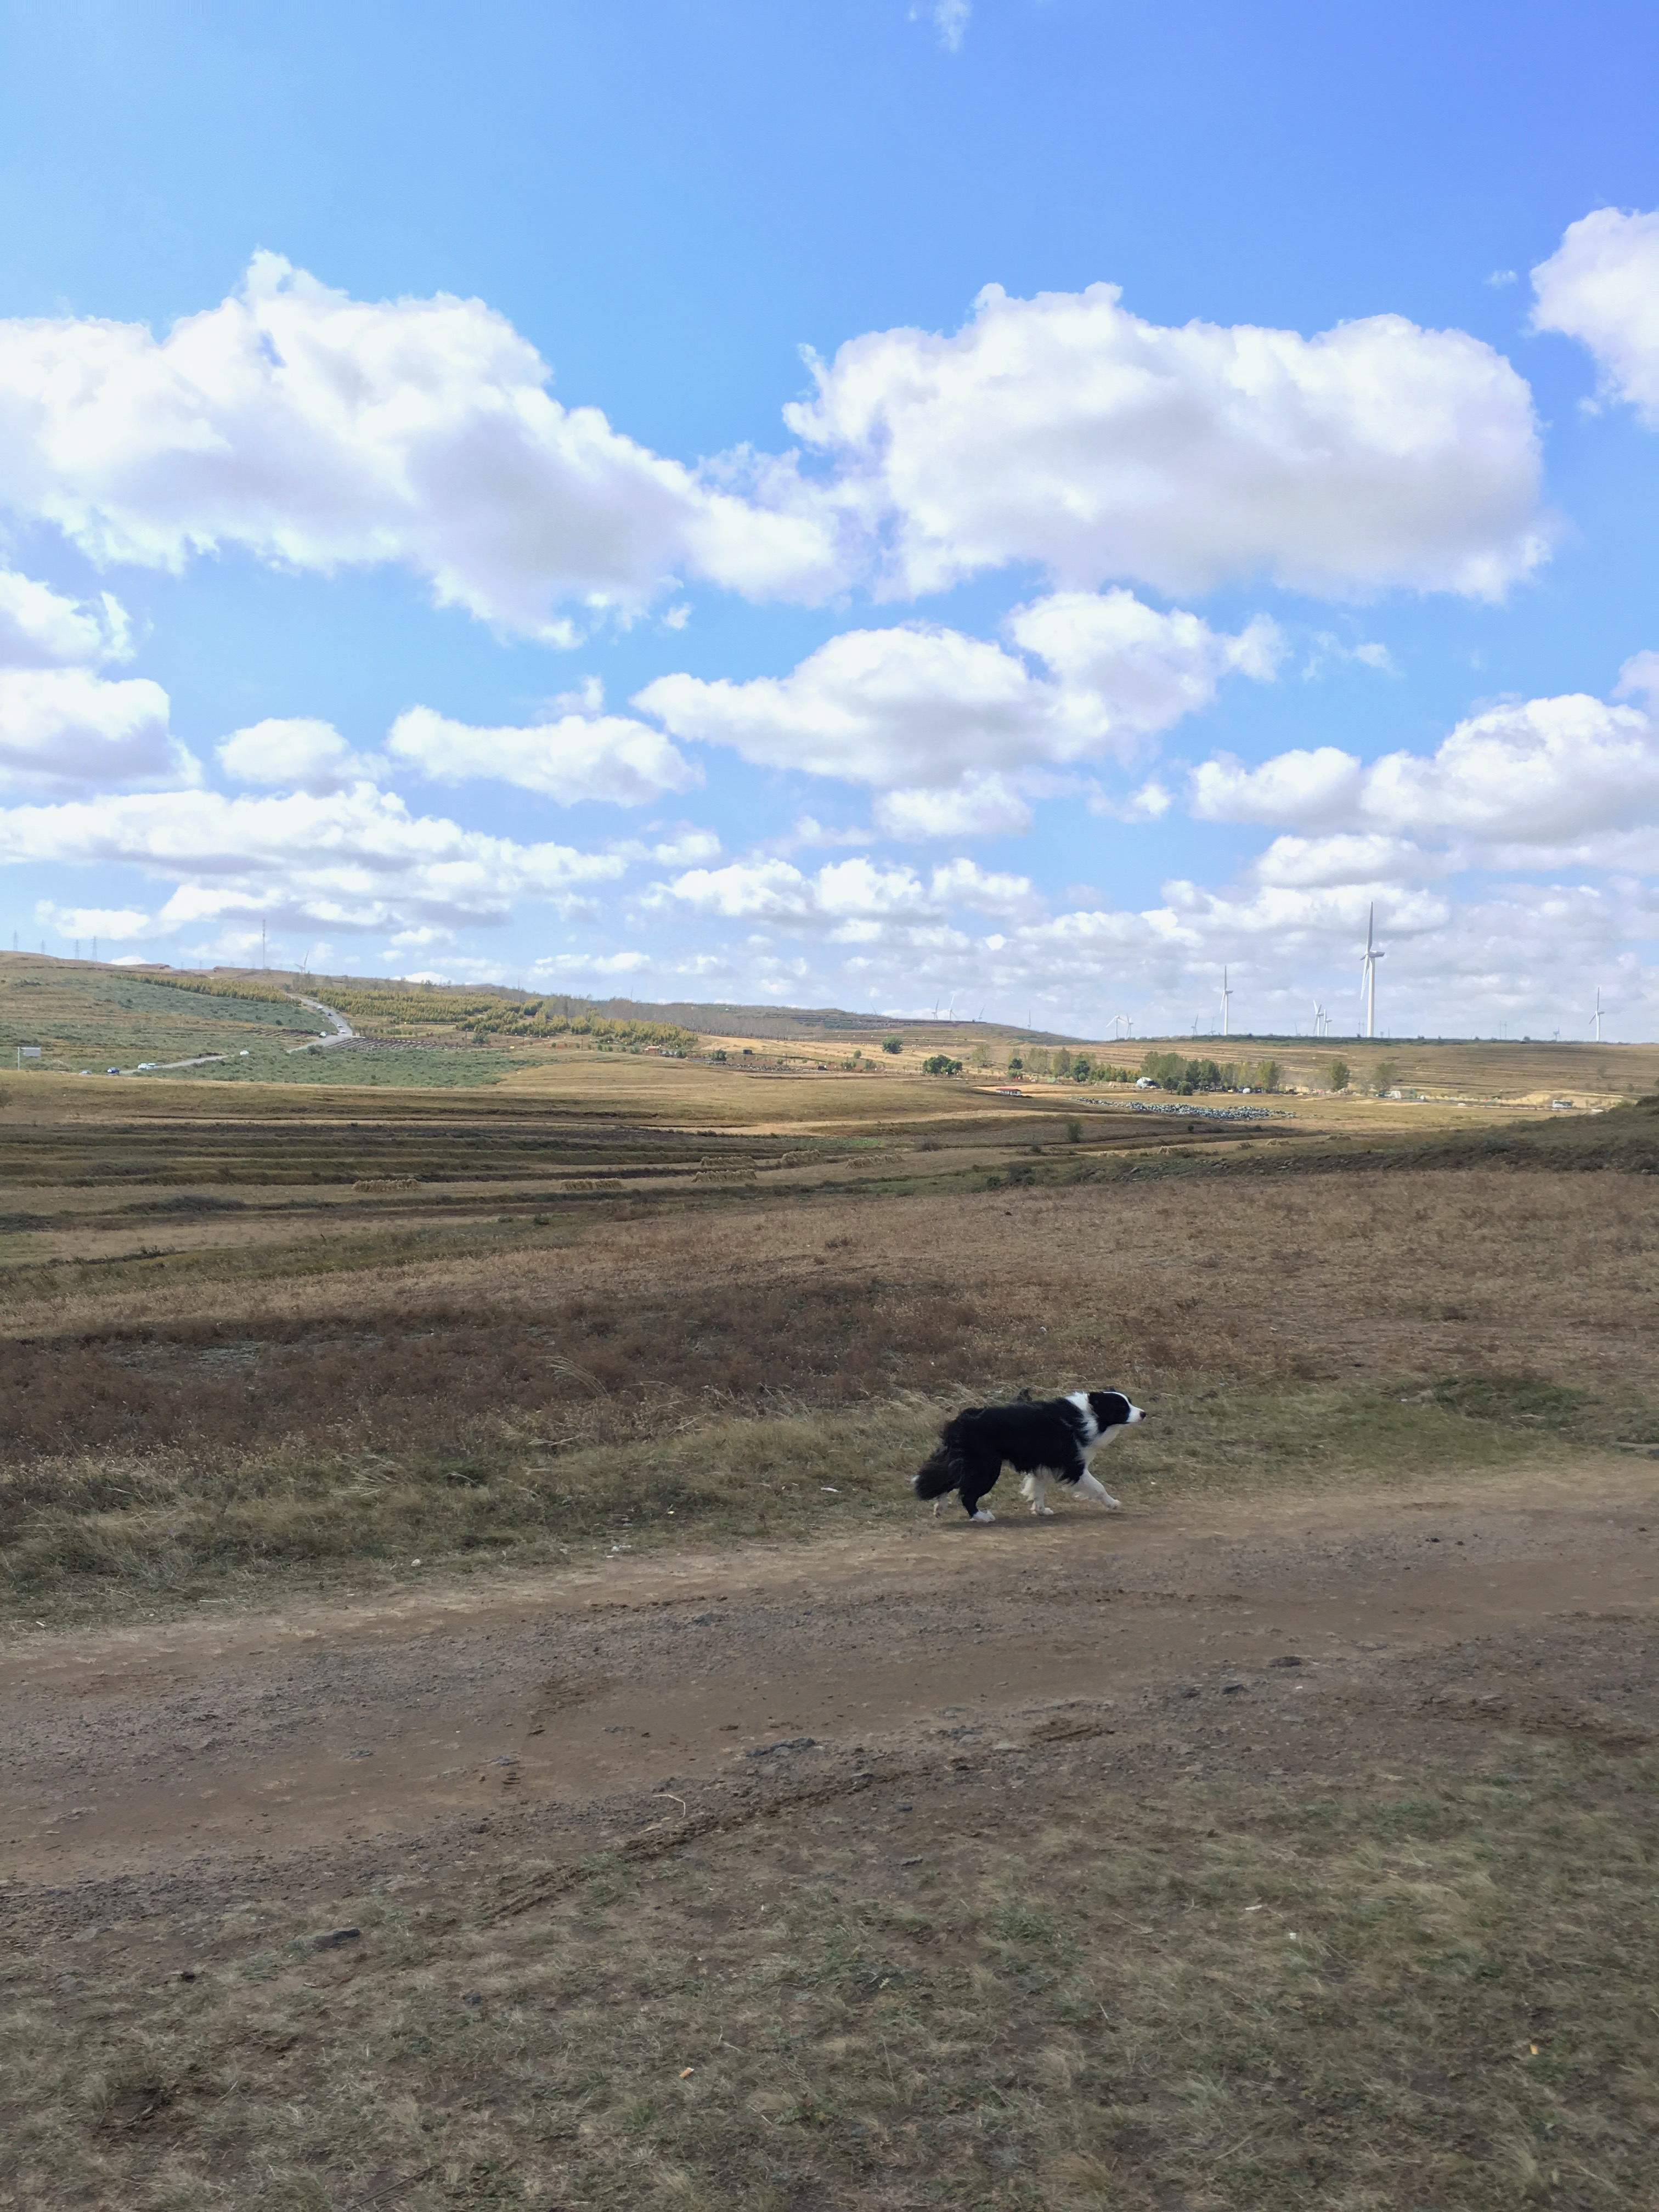
\includegraphics[width=1.00\paperwidth,height=\paperheight]{./alpha.jpeg}
	}
}
%% cf. manual of titlesec
\titleformat{\section}[block]{%
	\filcenter\large%
	\addtolength{\titlewidth}{2pc}%
%	\titleline*[c]{\titlerule*[.6pc]{\textbullet}}%
	\titleline*[c]{\titlerule*[0.6cm]{\lineornament{0.6cm}{0.30cm}{1}{70}}}%
	\addvspace{3pt}%
	\normalfont\bfseries}%
{\thesection}{1em}{}
\titlespacing{\section}{5pc}{*1}{0pt}[5pc]
% \def\fullsection#1#2#3{%
% 	\begin{center}
% 	{\large
% 	\lineornament{0.7cm}{0.3cm}{#3}{70}\\
% 	\phantomsection%
% 	\addcontentsline{toc}{section}{\protect\textbf{#1}}%
% 	{#1}
% 	\markboth{#2}{#1}%
% 	}%
% 	\end{center}
% }

%%% enhanced jigsaw:
%%  cf.~https://tex.stackexchange.com/questions/489714/transparency-option-in-tcolorbox
%%  and manual[10.11 Jigsaw Skin Variants]
%% Don't use \tcbox! Can't use \ht... in tcolorbox
% \newbox\clefhbox
% \setbox\clefhbox=\hbox{{\fontsize{36}{0}\selectfont\clefG}}
\def\clefGbox{
	\begin{tcolorbox}[width=3.5cm, square, circular arc, boxrule=0.5mm,
	       opacityframe=0.5, opacityback=0.3, enhanced jigsaw,
		colframe=MediumSpringGreen, colback=DodgerBlue,
		coltext=DarkViolet, halign=center, valign=center]
			{\fontsize{36}{0}\selectfont\clefG}
	\end{tcolorbox}
}
\def\titlebox#1#2{%
	\begin{tcolorbox}[beamer, width=0.7\hsize, arc=4mm,
		colframe=MediumSpringGreen, colback=DodgerBlue,
		coltext=white, halign=center, valign=center,
		halign lower=center, valign lower=center]
%		#1\\\vskip0.5cm\tcblower #2
		#1\\\vskip0.5cm #2
	\end{tcolorbox}
}
\def\datebox#1{
	\begin{tcolorbox}[arc = 3mm, boxrule=0.5mm, width=0.3\hsize,
	       opacityframe=0.5, opacityback=0.3, enhanced jigsaw,
		colback=MediumSpringGreen, colframe=DodgerBlue,
		coltext=white, halign=center, valign=center]
			#1
	\end{tcolorbox}
}
%% from manual tikz
\def\drawcallout#1#2#3{
\begin{tikzpicture}[remember picture, note/.style={ellipse callout, fill=LightSkyBlue}]
%	\draw [help lines] grid(17,3);
%	\node [note=red!50, callout relative pointer={(0,1)}] at (3,1) {Relative};
%	\node [note=blue!50, callout absolute pointer={(0,1)}] at (1,0) {Absolute};
	\node [draw, note=white, opacity=.5, overlay, callout relative pointer={#1}] at #2 {#3};
\end{tikzpicture}
}
%% copy from manual
\newcommand{\eachpageornament}{%
	\begin{tikzpicture}[remember picture, overlay]
	\node[anchor=north west, color=SlateBlue] at (current page.north west){%
		\pgfornament[width=0.8cm]{61}};
	\node[anchor=north east, color=SlateBlue] at (current page.north east){%
		\pgfornament[width=0.8cm,symmetry=v]{61}};
	\node[anchor=south west, color=SlateBlue] at (current page.south west){%
		\pgfornament[width=0.8cm,symmetry=h]{61}};
	\node[anchor=south east, color=SlateBlue] at (current page.south east){%
		\pgfornament[width=0.8cm,symmetry=c]{61}};
	\end{tikzpicture}%
}%
\newcount\pos
%% cf. manual
\newcommand{\lineornament}[4]{%
\begin{tikzpicture}[start chain,node distance=0,inner sep=0]
%	\node[minimum size=4pt,inner sep=0] (A) at (0,0){};
%	\coordinate (B) at (8,0);
	{%[start chain,node distance=0,inner sep=0]
	\node[anchor=west] [on chain] at (0, 0) {\pgfornament[height=#2,width=#1]{#4}};
%	\node [on chain] {\pgfornament[width=1cm]{70}};
%	\node [on chain] {\pgfornament[width=1cm]{70}};
%	\node [on chain] {\pgfornament[width=1cm]{70}};}
	\count\pos=1
	\loop
		\ifnum \count\pos < #3
			\node [on chain] {\pgfornament[height=#2,width=#1]{#4}};
			\advance\count\pos by 1
	\repeat
	}
\end{tikzpicture}%
}
% from https://tex.stackexchange.com/questions/167719/how-to-use-background-image-in-latex
\long\def\picbackground#1#2{%
\tikz[remember picture,overlay]
	\node[opacity=#2,inner sep=0pt] at (current page.center){%
	\includegraphics[width=\paperwidth,height=\paperheight]{#1}};%
}
% cf. https://tex.stackexchange.com/questions/519676/how-to-make-this-watermark
% https://tex.stackexchange.com/questions/527342/watermark-in-tikz-image
% https://texblog.org/2012/02/17/watermarks-draft-review-approved-confidential/
% https://www.latex4technics.com/?note=1c9f
% To use it,
% for example \awatermark{李小丹}{0.4}{45}{16}{gray}{current page.center}
% \long\def\awatermark#1#2#3#4#5#6{%
% \tikz[remember picture,overlay]
% 	\node[opacity=#2,inner sep=0pt,rotate=#3,scale=#4,color=#5] at (#6){%
% 	#1};%
% }

%% from manual
\definecolor{nicered}{rgb}{.647,.129,.149}
\makeatletter
\newlength\dlf@normtxtw
\setlength\dlf@normtxtw{\textwidth}
\def\myhelvetfont{\def\sfdefault{mdput}}
\newsavebox{\feline@chapter}
\newcommand\feline@chapter@marker[1][4cm]{%
\sbox\feline@chapter{%
	\resizebox{!}{#1}{\fboxsep=1pt%
	\colorbox{nicered}{\color{white}\bfseries\sffamily\thechapter}%
}}%
\rotatebox{90}{%
	\resizebox{%
		\heightof{\usebox{\feline@chapter}}+\depthof{\usebox{\feline@chapter}}}%
	{!}{\scshape\so\@chapapp}}\quad%
\raisebox{\depthof{\usebox{\feline@chapter}}}{\usebox{\feline@chapter}}%
}
\newcommand\feline@chm[1][4cm]{%
	\sbox\feline@chapter{\feline@chapter@marker[#1]}%
	\makebox[0pt][l]{% aka \rlap
	\makebox[1cm][r]{\usebox\feline@chapter}}}

\makechapterstyle{daleif1}{%
	\renewcommand\chapnamefont{\normalfont\Large\scshape\raggedleft\so}
	\renewcommand\chaptitlefont{\normalfont\Huge\bfseries\scshape\color{nicered}}
	\renewcommand\chapternamenum{}
	\renewcommand\printchaptername{}
	\renewcommand\printchapternum{\noindent\hfill\feline@chm[2.5cm]\par}
	%\renewcommand\afterchapternum{\par\vskip\midchapskip}
	\renewcommand\afterchapternum{\par}
	\renewcommand\printchaptertitle[1]{\chaptitlefont\hfill ##1\par}
}
\def\maketitle{%
%	\null
	\thispagestyle{empty}%
%%% from https://tex.stackexchange.com/questions/85904/showcase-of-beautiful-title-page-done-in-tex
	\BgThispage
	\begin{center}\leavevmode
		\clefGbox
%		\vskip6pt
%		\hrule height2pt\vskip2pt\hrule\vskip7pt
		\titlebox{{\Huge\textbf{乐谱集} \\}
		{\small\twoBeamedQuavers}{\large\youyuan{~五线谱~}}{\small\twoBeamedQuavers}}
		{{\large 李小丹\kern15pt 编著} \\ {\small\textit{\myemail}}}
	\end{center}
	\vskip6.3cm
	\noindent\drawcallout{(-0.5, -0.5)}{(13.4, 0)}%
		{{{\large\texttwemoji{musical note}}\ \youyuan 大王派我来巡山}}
	\vfill
	\begin{center}
		\datebox{{\small\bookver\\
		本书不定期更新...}}
	\end{center}
	\vskip2cm
	\hbox{}\hfill\ccby
%\null
	\cleardoublepage
}
\def\subtitlepage{%
	\picbackground{harmonica.jpeg}{0.2}
	\thispagestyle{empty}%
	\hbox{}\vskip10pt
	\begin{center}\leavevmode
		\vskip10pt
		\hrule height2pt\vskip2pt\hrule\vskip7pt
%		\lineornament{}{0.4cm}{1}{88}\\
		{{\Huge\textbf{乐谱集} \\}
		{\small\twoBeamedQuavers}{\large\youyuan{~五线谱~}}{\small\twoBeamedQuavers}}\\
		\vskip10pt
		{{\large 李小丹\kern8pt 编著}}
		\vskip5pt\hrule\vskip2pt\hrule height2pt\vskip7pt
	\end{center}
	\vskip6.3cm
	\vfill
	\begin{center}
		{\small\today\\}
		\lineornament{1cm}{0.4cm}{2}{71}
	\end{center}
	\vskip2cm
	\hbox{}\hfill\ccby
%\null
	\eject
}

% \pagestyle{fancy}
% \pagestyle{ruled}
% \fancyhead{} % clear all header fields
% \fancyfoot{} % clear all footer fields
% \fancyfoot[LE,RO]{\thepage}
% \fancyfoot[RE,LO]{\small\textsl{\rightmark}}
% \fancyhead[LE,RO]{\small\textsl{\rightmark}}
% \fancyhead[LO,RE]{\small\textsl{\leftmark}}
% \fancyhead[C]{\booked}
% \fancyfoot[C]{\hyperlink{chap:cont}{\faHandPointRight Go to Contents\faArrowCircleUp}}

\def\pagetopc{%
	\booked\kern0.3cm%
	{\LARGE\texttwemoji{dog2}\kern0.5cm%
	\texttwemoji{1f3c3-1f3fb-200d-2640-fe0f}%
	\texttwemoji{1f3c3-1f3fb-200d-2642-fe0f}}}

%%% cf. manual of memoir
\pagestyle{ruled}
% \makepagestyle{ruled}
% \makeevenhead{ruled}{{\small\textsl{\rightmark}}}{\booked}{{\small\textsl{\leftmark}}}
\makeevenhead{ruled}{{\small\textsl{\rightmark}}}{\pagetopc}{{\small\textsl{\leftmark}}}
% \makeoddhead{ruled}{{\small\textsl{\leftmark}}}{\booked}{{\small\textsl{\rightmark}}}
\makeoddhead{ruled}{{\small\textsl{\leftmark}}}{\pagetopc}{{\small\textsl{\rightmark}}}
\makeevenfoot{ruled}{{\small\thepage}}{\hyperlink{chap:cont}%
	{\faHandPointRight Go to Contents\faArrowCircleUp}}{{\small\textsl{\rightmark}}}
\makeoddfoot{ruled}{{\small\textsl{\rightmark}}}%
{\hyperlink{chap:cont}{\faHandPointRight Go to Contents\faArrowCircleUp}}{{\small\thepage}}
% \renewcommand{\headrulewidth}{0.4pt}
%\renewcommand{\footrulewidth}{0.4pt}

\newif\ifmark
\newif\ifmultimark
\long\def\epcall{%
	\eachpageornament%
	\global\marktrue%
	\global\multimarktrue%
%	\global\def\rightmark{}%
%	\global\def\leftmark{}%
}%

\renewcommand{\tocdataformat}[1]{%
	\normalfont{{\small(#1)~}}%
}
\long\def\pagemark#1#2{%
% FIXME
% Since markboth may have a bug,
% if next staff too big and markboth in a vbox, then it is invalid,
% and in this case, \TeX creates an empty page perhaps.
%	\markboth{#2}{#1}%
	\ifmark
		\global\def\rightmark{#1}%
		\global\def\leftmark{#2}%
		\markfalse%
	\else
		\ifmultimark
			\global\edef\rightmark{\rightmark,{$\noexpand\ldots$}}%
			\multimarkfalse%
		\fi%
	\fi%
}
\long\def\addsection#1#2{%
	\phantomsection%
	\addcontentsline{toc}{section}{\protect\textbf{#1}}%
	\section*{#1}%
	\pagemark{#1}{#2}
}%
\def\seclangtit#1{%
	\vskip-3pt%
	\noindent\hfil{\fontseries{semibold}\selectfont #1}\hfil\break%
	\vskip-7pt plus 3pt minus 10pt%
}

\def\submtitle#1{%
	\vskip-3pt%
	\noindent\hfil{\small #1}\hfil\break
	\vskip-7pt plus 3pt minus 10pt
}%

\def\composer#1{%
	\hbox to \hsize{\hfil #1}}

%%% 2023年 2月25日 星期六 13时23分46秒 CST
%%% author: Shao-Dan Lee 李小丹 字 殊恒

%%% FIXME Ugly! I don't know how call a macro of TeX in Lilypond,
%%% or define a macro by the code of lilypond.
% \def\book@edtion#1{%
% 	\lilypond[fragment,inline,staffsize=10]{
% 		\new Staff \with {
% 			\override Clef.color = "SlateBlue"}
% 		\relative {
% 			\override Staff.StaffSymbol.color = "FireBrick"
% 			\override NoteHead.color = "blue"
% 			\override Beam.color = "deepskyblue"
% 			\override Stem.color = "green"
% 			"#1"}}}%

\def\book@ed{%
	\lilypond[fragment,inline,staffsize=10]{
		\new Staff \with {
			\override Clef.color = "SlateBlue"}
		\relative {
			\override Staff.StaffSymbol.color = "FireBrick"
			\override NoteHead.color = "blue"
			\override Beam.color = "deepskyblue"
			\override Stem.color = "green"
			e'4. c8 [ f]}}}
\def\book@edd{%
	\lilypond[fragment,inline,staffsize=10]{
		\new Staff \with {
			\override Clef.color = "SlateBlue"}
		\relative {
			\override Staff.StaffSymbol.color = "FireBrick"
			\override NoteHead.color = "blue"
			\override Beam.color = "deepskyblue"
			\override Stem.color = "green"
			e'4. c8 [ f c]}}}%
\def\book@eddd{%
	\lilypond[fragment,inline,staffsize=10]{
		\new Staff \with {
			\override Clef.color = "SlateBlue"}
		\relative {
			\override Staff.StaffSymbol.color = "FireBrick"
			\override NoteHead.color = "blue"
			\override Beam.color = "deepskyblue"
			\override Stem.color = "green"
			e'4. c8 [ f c g']}}}%

\def\printbookver{%
\begin{tabu}{|[1pt]c|c|[1pt]}
	\tabucline[1pt]{1-2}
	Date & Edition \\\tabucline[1pt]{1-2}
	2023-02-03 & \book@ed\\\hline
	2023-02-03 & \book@edd\\\hline
	2023-12-21 & \book@eddd\\\tabucline[1pt]{1-2}
\end{tabu}
}
%%% XXX modify:
\let\booked=\book@eddd
\def\bookver{v3.6-$\beta$}
%\input{edition.tex}

%%% 2023年 2月16日 星期四 17时12分46秒 CST
%%% author: 李小丹(Shao-Dan Lee) 字 殊恒(Shuheng)

\renewcommand{\sharp}{\kern0.1em\lilyGlyph[scale=0.9,raise=1.1]{accidentals.sharp}}
\renewcommand{\flat}{\kern0.1em\lilyGlyph[scale=1.2,raise=0.8]{accidentals.flat}}

%%% FIXME: I don't know that call macro of tex in lilypond. Hence it is ugly!
\def\major@C{%
	\lilypond[fragment,inline,staffsize=11]{
		\new Staff \with {
			\override Clef.color = "blue"}
		\relative {
			\omit Staff.TimeSignature
			\override Staff.StaffSymbol.color = "blue"
			\override NoteHead.color = "blue"
			\override Beam.color = "deepskyblue"
			\override Stem.color = "green"
			s1}}}

\def\major@G{%
	\lilypond[fragment,inline,staffsize=11]{
		\new Staff \with {
			\override Clef.color = "blue"}
		\relative {
			\omit Staff.TimeSignature
			\override Staff.StaffSymbol.color = "blue"
			\override NoteHead.color = "blue"
			\override Beam.color = "deepskyblue"
			\override Stem.color = "green"
			\key g \major s1}}}
\def\major@D{%
	\lilypond[fragment,inline,staffsize=11]{
		\new Staff \with {
			\override Clef.color = "blue"}
		\relative {
			\omit Staff.TimeSignature
			\override Staff.StaffSymbol.color = "blue"
			\override NoteHead.color = "blue"
			\override Beam.color = "deepskyblue"
			\override Stem.color = "green"
			\key d \major s1}}}
\def\major@A{%
	\lilypond[fragment,inline,staffsize=11]{
		\new Staff \with {
			\override Clef.color = "blue"}
		\relative {
			\omit Staff.TimeSignature
			\override Staff.StaffSymbol.color = "blue"
			\override NoteHead.color = "blue"
			\override Beam.color = "deepskyblue"
			\override Stem.color = "green"
			\key a \major s1}}}
\def\major@E{%
	\lilypond[fragment,inline,staffsize=11]{
		\new Staff \with {
			\override Clef.color = "blue"}
		\relative {
			\omit Staff.TimeSignature
			\override Staff.StaffSymbol.color = "blue"
			\override NoteHead.color = "blue"
			\override Beam.color = "deepskyblue"
			\override Stem.color = "green"
			\key e \major s1}}}
\def\major@B{%
	\lilypond[fragment,inline,staffsize=11]{
		\new Staff \with {
			\override Clef.color = "blue"}
		\relative {
			\omit Staff.TimeSignature
			\override Staff.StaffSymbol.color = "blue"
			\override NoteHead.color = "blue"
			\override Beam.color = "deepskyblue"
			\override Stem.color = "green"
			\key b \major s1}}}
\def\major@FIS{%
	\lilypond[fragment,inline,staffsize=11]{
		\new Staff \with {
			\override Clef.color = "blue"}
		\relative {
			\omit Staff.TimeSignature
			\override Staff.StaffSymbol.color = "blue"
			\override NoteHead.color = "blue"
			\override Beam.color = "deepskyblue"
			\override Stem.color = "green"
			\key fis \major s1}}}
\def\major@CIS{%
	\lilypond[fragment,inline,staffsize=11]{
		\new Staff \with {
			\override Clef.color = "blue"}
		\relative {
			\omit Staff.TimeSignature
			\override Staff.StaffSymbol.color = "blue"
			\override NoteHead.color = "blue"
			\override Beam.color = "deepskyblue"
			\override Stem.color = "green"
			\key cis \major s1}}}
\def\major@AES{%
	\lilypond[fragment,inline,staffsize=11]{
		\new Staff \with {
			\override Clef.color = "blue"}
		\relative {
			\omit Staff.TimeSignature
			\override Staff.StaffSymbol.color = "blue"
			\override NoteHead.color = "blue"
			\override Beam.color = "deepskyblue"
			\override Stem.color = "green"
			\key aes \major s1}}}
\def\major@EES{%
	\lilypond[fragment,inline,staffsize=11]{
		\new Staff \with {
			\override Clef.color = "blue"}
		\relative {
			\omit Staff.TimeSignature
			\override Staff.StaffSymbol.color = "blue"
			\override NoteHead.color = "blue"
			\override Beam.color = "deepskyblue"
			\override Stem.color = "green"
			\key ees \major s1}}}
\def\major@BES{%
	\lilypond[fragment,inline,staffsize=11]{
		\new Staff \with {
			\override Clef.color = "blue"}
		\relative {
			\omit Staff.TimeSignature
			\override Staff.StaffSymbol.color = "blue"
			\override NoteHead.color = "blue"
			\override Beam.color = "deepskyblue"
			\override Stem.color = "green"
			\key bes \major s1}}}
\def\major@F{%
	\lilypond[fragment,inline,staffsize=11]{
		\new Staff \with {
			\override Clef.color = "blue"}
		\relative {
			\omit Staff.TimeSignature
			\override Staff.StaffSymbol.color = "blue"
			\override NoteHead.color = "blue"
			\override Beam.color = "deepskyblue"
			\override Stem.color = "green"
			\key f \major s1}}}
\def\major@CES{%
	\lilypond[fragment,inline,staffsize=11]{
		\new Staff \with {
			\override Clef.color = "blue"}
		\relative {
			\omit Staff.TimeSignature
			\override Staff.StaffSymbol.color = "blue"
			\override NoteHead.color = "blue"
			\override Beam.color = "deepskyblue"
			\override Stem.color = "green"
			\key ces \major s1}}}
\def\major@GES{%
	\lilypond[fragment,inline,staffsize=11]{
		\new Staff \with {
			\override Clef.color = "blue"}
		\relative {
			\omit Staff.TimeSignature
			\override Staff.StaffSymbol.color = "blue"
			\override NoteHead.color = "blue"
			\override Beam.color = "deepskyblue"
			\override Stem.color = "green"
			\key ges \major s1}}}
\def\major@DES{%
	\lilypond[fragment,inline,staffsize=11]{
		\new Staff \with {
			\override Clef.color = "blue"}
		\relative {
			\omit Staff.TimeSignature
			\override Staff.StaffSymbol.color = "blue"
			\override NoteHead.color = "blue"
			\override Beam.color = "deepskyblue"
			\override Stem.color = "green"
			\key des \major s1}}}

\def\circlefive{%
\begin{center}
	\begin{tikzpicture}[new set=import nodes]
		\begin{scope}[nodes={set=import nodes}]
			\node (a) at (0, 0) [ForestGreen, circle, draw, minimum size=0.36\vsize] {};
			\shade[shading=color wheel] [even odd rule]
			  (0,0) circle (0.182\vsize)
			  (0,0) circle (0.178\vsize);
		\end{scope}
		\graph[nodes = {draw, circle}, clockwise=12,
			tonic/.style={align=center, rectangle, minimum size=10mm,
				font=\footnotesize, very thick,draw=black!30,
				top color=yellow!20,bottom color=blue!20},
			outer/.style={minimum size=10mm, font=\footnotesize,
				very thick,draw=black!30, top color=red!20,bottom color=blue!20},
			inner/.style={minimum size=10mm, font=\small,
				very thick,draw=black!30, top color=blue!20,bottom color=green!20,}] {
		(import nodes);
		{ [name=in, radius=0.15\vsize] {"a"[inner], "e"[inner], "b"[inner], "f\,\sharp"[inner],
				"c\sharp"[inner], "g\sharp /a\flat"[inner], "d\sharp /e\flat"[inner],
				"a\sharp /b\flat"[inner], "f"[inner], "c"[inner], "g"[inner], "d"[inner]};},
		{ [name=out, radius=0.21\vsize] {"C"[outer], "G"[outer], "D"[outer], "A"[outer], "E"[outer],
				"B/C\flat"[outer], "F\sharp/G\flat"[outer], "C\sharp /D\flat"[outer],
				"A\flat"[outer], "E\flat"[outer], "B\flat"[outer], "F"[outer]};},
		{ [name=tonic, radius=0.28\vsize] {"\major@C"[tonic], "\major@G"[tonic], "\major@D"[tonic], "\major@A"[tonic],
			"\major@E"[tonic], "\major@B\\\major@CES"[tonic],
			"\major@FIS\\\major@GES"[tonic], "\major@CIS\\\major@DES"[tonic],
			"\major@AES"[tonic], "\major@EES"[tonic], "\major@BES"[tonic], "\major@F"[tonic],};}};
	\end{tikzpicture}
\end{center}
}%

\def\score@majorCIS{%
\begin{lilypond}
	\include "num_head.ly"
	\relative {
		\override Staff.Clef.full-size-change = ##t
		\key cis \major
		\time 4/4
		\easyHeadsOn
		cis'4 dis eis fis gis ais bis cis\bar "|."
	}
\end{lilypond}
}
\def\score@majorFIS{%
\begin{lilypond}
	\include "num_head.ly"
	\relative {
		\override Staff.Clef.full-size-change = ##t
		\key fis \major
		\time 4/4
		\easyHeadsOn
		fis'4 gis ais b cis dis eis fis\bar "|."
	}
\end{lilypond}
}
\def\score@majorB{%
\begin{lilypond}
	\include "num_head.ly"
	\relative {
		\override Staff.Clef.full-size-change = ##t
		\key b \major
		\time 4/4
		\easyHeadsOn
		b'4 cis dis e fis gis ais b\bar "|."
	}
\end{lilypond}
}
\def\score@majorE{%
\begin{lilypond}
	\include "num_head.ly"
	\relative {
		\override Staff.Clef.full-size-change = ##t
		\key e \major
		\time 4/4
		\easyHeadsOn
		e'4 fis gis a b cis dis e \bar "|."
	}
\end{lilypond}
}
\def\score@majorA{%
\begin{lilypond}
	\include "num_head.ly"
	\relative {
		\override Staff.Clef.full-size-change = ##t
		\key a \major
		\time 4/4
		\easyHeadsOn
		a'4 b cis d e fis gis a
		\bar "|."
	}
\end{lilypond}
}
\def\score@majorD{%
\begin{lilypond}
	\include "num_head.ly"
	\relative {
		\override Staff.Clef.full-size-change = ##t
		\key d \major
		\time 4/4
		\easyHeadsOn
		d'4 e fis g a b cis d
		\bar "|."
	}
\end{lilypond}
}
\def\score@majorG{%
\begin{lilypond}
	\include "num_head.ly"
	\relative {
		\override Staff.Clef.full-size-change = ##t
		\key g \major
		\time 4/4
		\easyHeadsOn
		g'4 a b c d e fis g
		\bar "|."
	}
\end{lilypond}
}
\def\score@majorC{%
\begin{lilypond}
	\include "num_head.ly"
	\relative {
		\override Staff.Clef.full-size-change = ##t
		\key c \major
		\time 4/4
		\easyHeadsOn
		c'4 d e f g a b c
		\bar "|."
	}
\end{lilypond}
}
\def\score@majorF{%
\begin{lilypond}
	\include "num_head.ly"
	\relative {
		\override Staff.Clef.full-size-change = ##t
		\key f \major
		\time 4/4
		\easyHeadsOn
		f'4 g a bes c d e f
		\bar "|."
	}
\end{lilypond}
}
\def\score@majorBES{%
\begin{lilypond}
	\include "num_head.ly"
	\relative {
		\override Staff.Clef.full-size-change = ##t
		\key bes \major
		\time 4/4
		\easyHeadsOn
		bes'4 c d ees f g a bes
		\bar "|."
	}
\end{lilypond}
}
\def\score@majorEES{%
\begin{lilypond}
	\include "num_head.ly"
	\relative {
		\override Staff.Clef.full-size-change = ##t
		\key ees \major
		\time 4/4
		\easyHeadsOn
		ees'4 f g aes bes c d ees
		\bar "|."
	}
\end{lilypond}
}
\def\score@majorAES{%
\begin{lilypond}
	\include "num_head.ly"
	\relative {
		\override Staff.Clef.full-size-change = ##t
		\key aes \major
		\time 4/4
		\easyHeadsOn
		aes'4 bes c des ees f g aes
		\bar "|."
	}
\end{lilypond}
}
\def\score@majorDES{%
\begin{lilypond}
	\include "num_head.ly"
	\relative {
		\override Staff.Clef.full-size-change = ##t
		\key des \major
		\time 4/4
		\easyHeadsOn
		des'4 ees f ges aes bes c des
		\bar "|."
	}
\end{lilypond}
}
\def\score@majorGES{%
\begin{lilypond}
	\include "num_head.ly"
	\relative {
		\override Staff.Clef.full-size-change = ##t
		\key ges \major
		\time 4/4
		\easyHeadsOn
		ges'4 aes bes ces des ees f ges
		\bar "|."
	}
\end{lilypond}
}
\def\score@majorCES{%
\begin{lilypond}
	\include "num_head.ly"
	\relative {
		\override Staff.Clef.full-size-change = ##t
		\key ces \major
		\time 4/4
		\easyHeadsOn
		ces'4 des ees fes ges aes bes ces
		\bar "|."
	}
\end{lilypond}
}
\def\score@minorais{%
\begin{lilypond}
	\include "num_head.ly"
	\relative {
		\override Staff.Clef.full-size-change = ##t
		\key ais \minor
		\time 4/4
		\easyHeadsOn
		ais'4 bis cis dis eis fis gis ais
		\bar "|."
	}
\end{lilypond}
}
\def\score@minordis{%
\begin{lilypond}
	\include "num_head.ly"
	\relative {
		\override Staff.Clef.full-size-change = ##t
		\key dis \minor
		\time 4/4
		\easyHeadsOn
		dis'4 eis fis gis ais b cis dis
		\bar "|."
	}
\end{lilypond}
}
\def\score@minorgis{%
\begin{lilypond}
	\include "num_head.ly"
	\relative {
		\override Staff.Clef.full-size-change = ##t
		\key gis \minor
		\time 4/4
		\easyHeadsOn
		gis'4 ais b cis dis e fis gis
		\bar "|."
	}
\end{lilypond}
}
\def\score@minorcis{%
\begin{lilypond}
	\include "num_head.ly"
	\relative {
		\override Staff.Clef.full-size-change = ##t
		\key cis \minor
		\time 4/4
		\easyHeadsOn
		cis'4 dis e fis gis a b cis
		\bar "|."
	}
\end{lilypond}
}
\def\score@minorfis{%
\begin{lilypond}
	\include "num_head.ly"
	\relative {
		\override Staff.Clef.full-size-change = ##t
		\key fis \minor
		\time 4/4
		\easyHeadsOn
		fis'4 gis a b cis d e fis
		\bar "|."
	}
\end{lilypond}
}
\def\score@minorb{%
\begin{lilypond}
	\include "num_head.ly"
	\relative {
		\override Staff.Clef.full-size-change = ##t
		\key b \minor
		\time 4/4
		\easyHeadsOn
		b'4 cis d e fis g a b
		\bar "|."
	}
\end{lilypond}
}
\def\score@minore{%
\begin{lilypond}
	\include "num_head.ly"
	\relative {
		\override Staff.Clef.full-size-change = ##t
		\key e \minor
		\time 4/4
		\easyHeadsOn
		e'4 fis g a b c d e
		\bar "|."
	}
\end{lilypond}
}
\def\score@minora{%
\begin{lilypond}
	\include "num_head.ly"
	\relative {
		\override Staff.Clef.full-size-change = ##t
		\key a \minor
		\time 4/4
		\easyHeadsOn
		a'4 b c d e f g a
		\bar "|."
	}
\end{lilypond}
}
\def\score@minord{%
\begin{lilypond}
	\include "num_head.ly"
	\relative {
		\override Staff.Clef.full-size-change = ##t
		\key d \minor
		\time 4/4
		\easyHeadsOn
		d'4 e f g a bes c d
		\bar "|."
	}
\end{lilypond}
}
\def\score@minorg{%
\begin{lilypond}
	\include "num_head.ly"
	\relative {
		\override Staff.Clef.full-size-change = ##t
		\key g \minor
		\time 4/4
		\easyHeadsOn
		g'4 a bes c d ees f g
		\bar "|."
	}
\end{lilypond}
}
\def\score@minorc{%
\begin{lilypond}
	\include "num_head.ly"
	\relative {
		\override Staff.Clef.full-size-change = ##t
		\key c \minor
		\time 4/4
		\easyHeadsOn
		c'4 d ees f g aes bes c
		\bar "|."
	}
\end{lilypond}
}
\def\score@minorf{%
\begin{lilypond}
	\include "num_head.ly"
	\relative {
		\override Staff.Clef.full-size-change = ##t
		\key f \minor
		\time 4/4
		\easyHeadsOn
		f'4 g aes bes c des ees f
		\bar "|."
	}
\end{lilypond}
}
\def\score@minorbes{%
\begin{lilypond}
	\include "num_head.ly"
	\relative {
		\override Staff.Clef.full-size-change = ##t
		\key bes \minor
		\time 4/4
		\easyHeadsOn
		bes'4 c des ees f ges aes bes
		\bar "|."
	}
\end{lilypond}
}
\def\score@minorees{%
\begin{lilypond}
	\include "num_head.ly"
	\relative {
		\override Staff.Clef.full-size-change = ##t
		\key ees \minor
		\time 4/4
		\easyHeadsOn
		ees'4 f ges aes bes ces des ees
		\bar "|."
	}
\end{lilypond}
}
\def\score@minoraes{%
\begin{lilypond}
	\include "num_head.ly"
	\relative {
		\override Staff.Clef.full-size-change = ##t
		\key aes \minor
		\time 4/4
		\easyHeadsOn
		aes'4 bes ces des ees fes ges aes
		\bar "|."
	}
\end{lilypond}
}

\def\tabmajorminor{%
%\begin{center}
%\setlength{\tabcolsep}{0pt}
\begin{longtabu}{|[2pt]c|r|[1pt]c|r|[2pt]}
	\tabucline[2pt]{1-4}
	\multicolumn{2}{|[2pt]c}{大调} & \multicolumn{2}{c|[2pt]}{自然小调}\\\tabucline[1pt]{1-4}
	C\sharp & \score@majorCIS & a\sharp & \score@minorais\\\hline
	F\sharp & \score@majorFIS & d\sharp & \score@minordis\\\hline
	B & \score@majorB         & g\sharp & \score@minorgis\\\hline
	E & \score@majorE         & c\sharp & \score@minorcis\\\hline
	A & \score@majorA         & f\sharp & \score@minorfis\\\hline
	D & \score@majorD         & b & \score@minorb\\\hline
	G & \score@majorG         & e & \score@minore\\\hline
	C & \score@majorC         & a & \score@minora\\\hline
	F & \score@majorF         & d & \score@minord\\\hline
	B\flat & \score@majorBES  & g & \score@minorg\\\hline
	E\flat & \score@majorEES  & c & \score@minorc\\\hline
	A\flat & \score@majorAES  & f & \score@minorf\\\hline
	D\flat & \score@majorDES  & b\flat & \score@minorbes\\\hline
	G\flat & \score@majorGES  & e\flat & \score@minorees\\\hline
	C\flat & \score@majorCES  & a\flat & \score@minoraes\\\tabucline[2pt]{1-4}
\end{longtabu}
% \begin{longtabu}{|[2pt]c|r|[2pt]}
% 	\tabucline[2pt]{1-2}
% 	\multicolumn{2}{|[2pt]c|[2pt]}{自然小调}\\\tabucline[1pt]{1-2}
% 	a\sharp & \score@minorais\\\hline
% 	d\sharp & \score@minordis\\\hline
% 	g\sharp & \score@minorgis\\\hline
% 	c\sharp & \score@minorcis\\\hline
% 	f\sharp & \score@minorfis\\\hline
% 	b & \score@minorb\\\hline
% 	e & \score@minore\\\hline
% 	a & \score@minora\\\hline
% 	d & \score@minord\\\hline
% 	g & \score@minorg\\\hline
% 	c & \score@minorc\\\hline
% 	f & \score@minorf\\\hline
% 	b\flat & \score@minorbes\\\hline
% 	e\flat & \score@minorees\\\hline
% 	a\flat & \score@minoraes\\\tabucline[2pt]{1-2}
% \end{longtabu}
%\end{center}
}%


\def\emptypage{%
\thispagestyle{empty}
\nopagecolor%
%% from manual latexsource2e
\RemoveFromHook{shipout/background}%
}%
%\newcount\pg
\long\def\make@emptypage{%
	\emptypage
	\hbox{}\vfill\eject}
\long\def\makeemptypage#1{%
	\count100=#1
	\ifnum\count100>0
	\make@emptypage
	\advance\count100 by -1
	\makeemptypage{\the\count100}
	\relax
	\else
	\relax
	\fi%
}%

%%% bug in tabu when rowcolors are defined?
%%% cf. https://tex.stackexchange.com/questions/36089/bug-in-tabu-when-rowcolors-are-defined#:~:text=colorlet%20%7Bheadcolor%7D%20%7Bgray%2125%7D%20begin%20%7Btabu%7D%20to%200.8textwidth%20%7BX,width%20of%20the%20column%20%5C%20hline%20end%20%7Btabu%7D
%%% \rowfont{...}\rowcolor{...} is ok?
%%% the following code isn't ok, not compatible with multirow
%%% \def\tbhcolor{%
%%%	\taburowcolors 1{LightSeaGreen .. LightSeaGreen}}
%%% \def\tbbcolor{%
%%%	\taburowcolors 1{white .. white}}
%%% so I use colorbox:
\def\tbhcolor#1{%
	\colorbox{LightSkyBlue}{\hbox to 0.94\hsize{\hss#1\hss}}}

\newcommand{\eg}{e.g.,} %% for example
\def\thecoda{\kern3pt\lilyGlyph[scale=1.4,raise=0.5]{scripts.coda}}
\def\thesegno{\kern3pt\lilyGlyph[scale=1.1,raise=0.5]{scripts.segno}}
\def\thestopped{\lilyText[scale=1.5]{+}}
\def\theharmonic{\lilyGlyph[raise=0.5]{noteheads.s0harmonic}}
\def\theflageolet{\kern2pt\lilyGlyph[raise=0.5]{scripts.flageolet}}
\def\thefermata{\kern2pt\fermata}
\def\thesnap{\kern2pt\lilyGlyph[raise=0.5,scale=1.2]{scripts.snappizzicato}}
\def\tllangle{\hbox{$\langle\!\langle$}}
\def\trrangle{\hbox{$\rangle\!\rangle$}}

\newif\ifdebug
\debugfalse
% \debugtrue

%%% from https://github.com/EagleoutIce/fancyqr/
%%% https://github.com/EagleoutIce/fancyqr/blob/main/qr-example.tex
%%% cf. manual qrcode
\def\qr@code#1#2{%
% \FancyQrDoNotPrintSquare{8}{9}
% \FancyQrHardCut
	\fancyqrset{level=H}%
	\FancyQrLoad{glitch}%
	\fancyqr[image=#1]{#2}}%

\def\theqr#1#2#3{%
\ifdebug
	\relax
\else
	\setbox100=\hbox{\qr@code{#1}{#2}}
	\setbox101=\hbox{#3}
	\dimen100=\wd100
	\ifnum \wd100 < \wd101
		\dimen100=\wd101
	\fi%
	\vbox{%
		\hbox to \dimen100{\hfil\unhbox100\hfil}
		\hbox to \dimen100{\hfil\unhbox101\hfil}}\fi}%

\makeatother


\begin{document}

\chapterstyle{daleif1}
\marktrue
\multimarktrue

\maketitle
\subtitlepage

\thispagestyle{empty}
{\obeylines\parindent=0pt\smallskip
\textcopyright 2023,2024 李小丹
本书采用\ccby 协议进行授权。
\texttwemoji{e-mail}\ \myemail
\href{https://shuhenglee.github.io}%
{\texttwemoji{link}\ https://shuhenglee.github.io}
%\href{https://leeshuheng.wordpress.com}%
%{\faWordpress https://leeshuheng.wordpress.com}
\href{https://github.com/shuhenglee/score\_set}%
{\kern-4pt\faGithub https://github.com/shuhenglee/score\_set}
\href{https://github.com/shuhenglee/tex\_score\_set}%
{\kern-4pt\faCode https://github.com/shuhenglee/tex\_score\_set}
\bigskip
本书内容适合玩小提琴或14孔半音阶口琴的新手。\bigskip}

\noindent\printbookver
\vfill
\hfill\theqr{\faGithub}%
{https://raw.githubusercontent.com/shuhenglee/score_set/main/score_set.pdf}{扫码下载本书}
\eject

% cf. manual latexsource2e
% cf. manual everypage
% cf. manual ltshipout
% cf. https://www.latex-project.org//news/2020/10/01/issue32-of-latex2e-released/
% cf. https://tex.stackexchange.com/questions/615010/how-can-i-use-latex-hooks-in-historical-versions-of-tex-live
%\AddEverypageHook{⟨code⟩} ≡ \AddToHook{shipout/background}{\put(1in,-1in){⟨code ⟩}}
\AddEverypageHook{\epcall}

\frontmatter

\chapter{Preface}
我把演奏某种乐器作为爱好,主要是缘于上小学时教我音乐的于老师以及
教我小提琴的郭老师。因为一些书买不到,
当初我的好多提琴谱都是郭老师一笔一笔抄出来的,非常辛苦。
郭老师和于老师是我童年时代最好的老师。
最近我学习半音阶口琴,也想手抄一些乐谱。
但由于比较费手和钢笔水,所以果断放弃手写。
而且我的夫人小叶子正好买了一台打印机,
巧的是我有一台电脑,更巧的是这台电脑上刚好有编辑排版的软件。
末页那张风信子的照片也是小叶子拍摄的。

本书使用\LaTeX (\TeX\ Live 2022\footnote{现已升级至\TeX\ Live 2024})
和lilypond-book(GNU LilyPond 2.24.0\footnote{现已升级至GNU LilyPond 2.24.4})排版,
使用vim编写前两者的脚本。\LaTeX 和vim都是我十几年的老朋友了。
这些软件一如既往的优秀是本书能够成功排版的关键。
十几年前,我想在Sun贡献的OpenOffice上写文章,但我放弃了。
因为\LaTeX 已足够,而且\LaTeX 可以与vim相互配合。
vim的祖宗vi是Sun的首席科学家创建的,看来我并没有绕开Sun.
\LaTeX 是\TeX 的一个format,而\TeX 是计算机科学家高德纳老先生创造的。
作为排版软件,\TeX 非常强大。LilyPond是我的新朋友,通过这几天
的使用,发现LilyPond排版五线谱非常好用。
我选择LilyPond是因为她基于\TeX 并与\LaTeX 兼容,
而且语法相对简单。
从她的构成来看,感觉LilyPond更像是lisp和\TeX 的混合体。
我很多年前学过Common Lisp,但因为没有使用她,就忘光了。
lisp也是老古董了!LilyPond毕竟是GNU的东西,有lisp是很正常的。
再说,我也有点儿Oldschool风格。
当然,即使不会lisp和\TeX ,也可以使用LilyPond排版各种乐谱,
LilyPond可以单独使用。

我们家的小狗狗对本书亦有贡献。
Alpha\texttwemoji{dog face}极不情愿、勉为其难的贡献
出自己的照片作为本书的封面,作为报复,Alpha在我编写代码的
过程中不断使用它的毛来攻击我的电脑,
如果没有小叶子的鼓励和支持,我可能早就被Alpha打败了。
Alpha不是老派的狗狗,它既不会在
月圆之夜伏案计算下列级数
\begin{equation*}
	1 - \frac{1}{3} + \frac{1}{5} - \frac{1}{7} + \frac{1}{9} - \cdots,
\end{equation*}
然后夺门而出、狂奔到荒无人烟的山顶,以该级数的结果
为角度抬起狗头仰天长啸;
也不会在凌晨四点半被闹钟叫醒,跑去浓雾弥漫的牧场当羊倌,去伺候那些由于毛发浓密而不愿奔跑的绵羊,
却又任凭自己的狗毛不断脱落。
落草为寇和社畜的生活它都不喜欢。除排泄外,Alpha只想
静静地躺在家里,有酸奶喝便是极好的。然后用它的狗毛占领全宇宙。
如果十几万年以后的人类在距离地球几万光年的类地行星
上发现Alpha的毛,我是不会感到惊讶的。
引力无法阻止Alpha的毛,
牛顿、爱因斯坦、波尔、海森堡、波恩、薛定谔、狄拉克、泡利、
费曼、杨振宁、李小丹、埃伦费斯特、吴健雄、朗道、
孙悟空、白素贞、尔康等
你能列举的任何物理学家所发现的定理,
以及寒暑假的任何大神都无法阻止Alpha的毛。
它的毛是漫威宇宙遗留在人类世界的产物。

%%% FIXME
本书更新可在%
\href{https://github.com/shuhenglee/score\_set}%
{\faGithub https://github.com/shuhenglee/score\_set}
免费下载。该网站经常连不上,连上了也不一定能下载,能下载了速度也很慢。
总之,就是能不能下载看缘份。另外,本书所包含曲目都提供了MIDI,
可在上述网站免费下载。本书的\LaTeX{}源码下载地址:

\href{https://github.com/shuhenglee/tex\_score\_set}%
{\kern-4pt\faCode https://github.com/shuhenglee/tex\_score\_set.}

本书将不定期更新...

由于编者乐理知识的欠缺,而且还需要抵御大量狗毛袭击,
本书不可避免的存在一些错误且更新较慢;
某些曲谱是我小时候学习小提琴用的,为了适应我初学者的水平,
郭老师对曲谱进行了修改;
又由于编者比较懒,所以在乐谱中省略了较长的前奏和间奏,请凑合着演奏。
\vfil\break

\pagecolor{Cornsilk} %pagecolor from this page.
\hypertarget{chap:cont}{}
\tableofcontents
\vfill\break

\mainmatter

%%% ============================
\chapter{民歌}

\circlefive
\vfil\break

%%% 2023年 2月14日 星期二 11时18分26秒 CST
%%% author: Shao-Dan Lee 李小丹 字 殊恒

\hbox{}\vskip0pt plus 1fil

\addsection{五月之歌}{民歌}
\seclangtit{May Song}

~\hfill{\youyuan 民歌}

\begin{lilypond}
\layout {
	indent = #0
	line-width = #164
 	\context {%
 		\Score
 		\override SpacingSpanner.base-shortest-duration = #(ly:make-moment 1 16)
 	}
}
\score{
\relative {%
	\set Score.barNumberVisibility = #all-bar-numbers-visible
	%\override Score.BarNumber.break-visibility = #all-visible
	\override Score.BarNumber.break-visibility = #end-of-line-invisible
	\tempo "Allegro Moderato"
	\key a \major
	\time 4/4
	\repeat volta 2 {a'4.\downbow cis8\upbow e4 a fis a8 fis e2
	d4. e8 cis4 a b2 a e'4 e d d
	cis\mf e8 cis\> b2 e4\p e d d cis e8 cis b2
	a4.\f cis8 e4 a fis a8 fis e2
	d4. e8 cis4 a b2_\markup{\italic{\teeny{2da volta poco rit.}}} a}
}%
\layout { }
%\midi { }
}
\end{lilypond}
\vskip0pt plus 1fil

%%% 2023年 2月 2日 星期四 12时08分15秒 CST
%%% author: Shao-Dan Lee 李小丹 字 殊恒

\addsection{红河谷}{民歌}

~\hfill{\youyuan 加拿大民歌}

\begin{lilypond}
\layout {
	indent = #0
	line-width = #164
 	\context {%
 		\Score
 		\override SpacingSpanner.base-shortest-duration = #(ly:make-moment 1 16)
 	}
}
\score {
\relative {%
	\set Score.barNumberVisibility = #all-bar-numbers-visible
	%\override Score.BarNumber.break-visibility = #all-visible
	\override Score.BarNumber.break-visibility = #end-of-line-invisible
	\tempo "Moderato"
	\key c \major
	\time 4/4
	\partial 4 g'8 c e4 e8 e e4 d8 e d c ( c2) g8 c
	e4 c8 e g4 f8 e d2. g8 f e4 e8 d c4 d8 e g f ( f2)
	a,8 aes g4 b8 c d4 e8 d c2. r4 \bar "|."
}%
\layout { }
%\midi { }
}
\end{lilypond}
\vskip0pt plus 1fil

%%% 2023年 2月 2日 星期四 12时20分39秒 CST
%%% author: Shao-Dan Lee 李小丹 字 殊恒

\addsection{夏日最后一朵玫瑰}{民歌}

~\hfill{\youyuan 爱尔兰民歌}

\begin{lilypond}
\layout {
	indent = #0
	line-width = #164
 	\context {%
 		\Score
 		\override SpacingSpanner.base-shortest-duration = #(ly:make-moment 1 16)
 	}
}
\score {
\relative {%
	\set Score.barNumberVisibility = #all-bar-numbers-visible
	%\override Score.BarNumber.break-visibility = #all-visible
	\override Score.BarNumber.break-visibility = #end-of-line-invisible
	\tempo "Moderato"
	\key c \major
	\time 3/4
	\partial 4 c''8. ( d16) e4 c'8. \> ( b16) a8. ( g16)
	g8 ( e4.) \! c8. ( d16) e8 ( g4) e8 d8.( c16) c4. r8 c8. ( d16)
	e4 c'8. ( b16) a8. ( g16) g8 ( e4.) c8. ( d16)
	e8 ( g4) e8 d8. ( c16) c4. r8 g'8. ( e16)
	c'4. ( b8) a8. ( g16) g4 ( e) g8. ( e16)
	c'4. ( b8) a8 [( gis)] a8. \< ( b16) c4^\fermata \! c,8. ( d16)
	e4 c'8. ( b16) a8. ( g!16) g8 ( e4.) c8. ( d16)
	e8 ( g4) e8 \> d8. ( c16) c2 \! r4 \bar "|."
}%
\layout { }
%\midi { }
}
\end{lilypond}
\vskip0pt plus 1fil\break

%%% 2023年 2月 3日 星期五 15时23分21秒 CST
%%% author: Shao-Dan Lee 李小丹 字 殊恒

\leavevmode\vfil%
\addsection{小红帽}{民歌}
\vbox{% To prevent page break
\vskip-10pt\composer{{\youyuan 巴西民歌}}
\begin{lilypond}
\layout {
	indent = #0
	line-width = #164
 	\context {%
 		\Score
 		\override SpacingSpanner.base-shortest-duration = #(ly:make-moment 1 16)
 	}
}
\score{
\relative {%
	\set Score.barNumberVisibility = #all-bar-numbers-visible
	%\override Score.BarNumber.break-visibility = #all-visible
	\override Score.BarNumber.break-visibility = #end-of-line-invisible
	\tempo "Allegreto"
	\key c \major
	\time 2/4
	c''8 d e f g4 e8 c
	c'4 a8 f g g e4
	c8 d e f g e d c
	d4 e d g
	c,8 d e f g4 e8 c c'4 a8 f g4 e
	c8 d e f g e d c
	d4 e c c
	c'4 a8 f g g c,4
	c'4 a8 f g4 e c8 d e f g e d c
	d4 e c c \bar "|."
}%
\layout { }
%\midi { }
}
\end{lilypond}
\addsection{友谊地久天长}{民歌}
\vskip-10pt\composer{{\youyuan 苏格兰民歌}}
\begin{lilypond}
\layout {
	indent = #0
	line-width = #164
 	\context {%
 		\Score
 		\override SpacingSpanner.base-shortest-duration = #(ly:make-moment 1 16)
 	}
}
\score {
\relative {%
	\set Score.barNumberVisibility = #all-bar-numbers-visible
	%\override Score.BarNumber.break-visibility = #all-visible
	\override Score.BarNumber.break-visibility = #end-of-line-invisible
	\tempo "Moderato cantabile"
	\key c \major
	\time 4/4
	\partial 4 d'\mp g4. g8 g4 b a4. g8 a4 b g4.\< g8 b4 d e2\mf r4 e
	d4. b8 b4 g a4. g8 a4 b g4.\> e8 e4 d | g2\! r4 e'\mp
	d4. b8 b4 g a4. g8 a4 e' d4.\< b8 b4 d e2\! r4 g\mp
	d4. b8 b4 g a4. g8 a4 b8 ( a) g4. e8\> e4 d g2.\p \bar "|."
}%
\layout { }
%\midi { }
}
\end{lilypond}
\addsection{茉莉花}{民歌}
\vskip-10pt\composer{{\youyuan 江苏民歌}}
\begin{lilypond}
\include "conf.ly"
\score {
\relative {%
	\key f \major
	\time 2/4
	\tempo "Allegretto cantabile"
	a'16( g a c) d( c f d) c( a c4 d8)
	f( g16 a) g( f d f) c2
	c16( a c4 d8) f( g16 a) g( f d8)
	c( g) a16( c a g) f( d f4.)
	a16( g f8) g8.( a16) c8( d16 f) d8( c)
	c16( a g8) a16( c a g) f( g d4 f8)
	g8.( a16) f( g f d) f( d c4.)
	a'16( g f8) g8.( a16) c8( d16 f) d8( c)
	c16( a g8) a16( c a g) f( g d4 f8)
	g'8.( a16) f( g f d) c_\markup{\small\italic{rit.}}( d f a g f d f)
	c2\>\fermata \bar "|."\!
}%
\layout { }
%\midi { }
}
\end{lilypond}}
\vfil\eject

%%% 2023年12月27日 星期三 08时41分37秒 CST
%%% author: Shao-Dan Lee 李小丹 字 殊恒
\hbox{}\vfill %it is invalid to use \noindent
%\tocdata{toc}{}
\addsection{步步高}{民歌}
\composer{{\youyuan 广东乐曲}}
%\composer{R.~Schumann}
\begin{lilypond}
\include "conf.ly"
\score {
\relative {%
	\tempo "Moderato"
	\key c \major
	\time 2/4
	e'8[ e] g r g'\upbow( e) d16 e c d
	a8[ c] g16[ a g8]
	r8 e16\upbow( g) d8 e
	g8 e16( g) c8 e, g4 f16\upbow g e8
	f16 g e8 d16( e g a)
	c,4. d16\upbow( e)
	c8 d16( e) c8 d16( e) c8[ c] r8 d\upbow
	e16 d e4 g8\upbow a8[ c] g16[ a f8]
	e16\upbow d e4( g8)
	d'4.\downbow e8 d16 e d c a c d e
	c8 r16 a,\upbow g8 a
	c[ a16 c] g8[ c] c r
	c'\upbow[ a16 g] e g a c g4
	g8 r c,16\downbow[ d e8]
	d e c16\downbow[ d e8]
	d[ e] g[ e16( d)] c8 b c4
	c8\upbow[ g16 a] c8 d
	e16 d e4 g8 c b a g e' e r d\upbow
	c4 c8 r d8( e16 d) c4 d8( e16 d) c4
	e16 d c d e d c d e g e d c4
	c8\upbow a16 c g8 e
	r8 a\upbow g[ f] e d c d
	e a, b d e16 d e4 a16( g)
	e8 g4( a8) g g4( a16 c)
	g8 g4( d'16 e) c8 c4( e16 d)
	c8 c4( d8) e16 d e4 d8 e d e g
	d c b a g g4( a16 g)
	f8 g4( f8) g4 g8[ e16 d]
	c d e g d8 g, c r c'8.\upbow( b16)
	a8 a g8. a16 e8 e f8. e16 d8 d e8. d16
	c8[ g16( a)] c8 c c[ c16( e)] g8 g
	g[ c16( a)] g c a g
	e8[ d16( e)] d16[ c8( d16)]
	e8. d16 e8 g a b c16 d e d c4 c8 r \fine
}
\layout { }
% \midi { }
}
\end{lilypond}

\vfill\break

%%% 2023年12月28日 星期四 10时37分32秒 CST
%%% author: Shao-Dan Lee 李小丹 字 殊恒

\hbox{}\vfill %it is invalid to use \noindent
\tocdata{toc}{聂耳}
\addsection{金蛇狂舞}{民歌}
%\seclangtit{The Two Grenadiers}
\composer{聂耳}
\begin{lilypond}
\include "conf.ly"
\score {
\relative {%
	\tempo "Allegro"
	\key g \major
	\time 2/4
	\partial 4 e'8 g d e g4 d'8.\upbow( e16) c8 b a4
	a8\upbow( d) d a c b a[ g16( a)] c8 c e, g
	a c a16( g e g ) d4 e8 e d4
	d'8\downbow d c c d d a4
	a8( d) c c e, g a4 c8\upbow( a) a c
	d4 d8( e) g4 e8( g) g e d4
	d8\upbow( e) d c a4 a8( d)
	d a c b a[ g16( a)] c8 c
	e, g a c a16( g e g) d4 e8 e d4
	d'8\downbow e d e d c d4
	g,8.\downbow a16 g8 a d, e g4
	d'8.\downbow e16 d8 e g e d4
	g,8.\downbow a16 g8 a d, e g4
	d'8\downbow e d c \partial 4 d4
	g,8.\downbow a16 d,8 e \partial 4 g4
	\repeat unfold 2 { d'8\downbow e d4 g,8\downbow a g4}
	\repeat unfold 2 { d'8\downbow r g,\upbow r }
	d'8 d g, d' g, d' g, d'
	\repeat unfold 2 { g, r g r }
	g g g g r g\upbow[ g\downbow] r
	d'8\downbow d c c d d a4
	a8\upbow( d) c c e, g a4
	c8\upbow( a) a c d d d e
	g g e g g e d4 d8\upbow( e) d c
	a4 a8\upbow( d) d a c b a[ g16( a)] c8 c
	e, g a c a16( g e g) d4 e'8 e d r \fine
}
\layout { }
% \midi { }
}
\end{lilypond}

\vfill\break

%%% 2024年 1月 2日 星期二 08时46分32秒 CST
%%% author: Shao-Dan Lee 李小丹 字 殊恒

\hbox{}\vfill %it is invalid to use \noindent
%\tocdata{toc}{}
\addsection{花儿与少年}{民歌}
\composer{{\youyuan 青海民歌}}
%\composer{R.~Schumann}
\begin{lilypond}
\include "conf.ly"
\score {
\relative {%
	\tempo "Moderato cantabile"
	\key a \minor
	\time 2/4
	\repeat segno 2 {\repeat volta 2 {e''8\downbow a e16 g e d e d c b a4
		\repeat unfold 2 {a'8\upbow a16 b a g e g a2}
		a8 a d a16 g a8 a g e a a16 b a g e8
		d8. e16 g16 a g e d8 e16 g e d c b a2
		\repeat unfold 2 {a'8 a16 b a g e8 d4 d}
		a'8[ a16 b] a g e8 d8. e16 g a g e
		d8 e16 g e d c b \bar "|"}}
	\alternative {
		\volta 1 {
			\alternative {
				\volta 1 {a2 \bar ":|."}
				\volta 2 {\time 3/4 \tempo "Allegro cantabile" a2. ~a}}
			\repeat volta 2 {
			a,2^\markup{\italic{\teeny{2da volta 8va.}}}\downbow( c4) a2( c4)
			d4( c d) e4.( d8 e[ g]) a2. ~a
			a4.( c8 a[ g]) e2( g4) a( e g)
			d( c d) e2. ~e a4( e g)
			d( c d) e2( d8 c) d2( a4)
			a( c d) e4.( g8 d[ c]) d2( e4)
			a,4( c d8 e) d2( c4)}
			\alternative {
				\volta 1 {a2. ~a}
				\volta 2 {\time 2/4 {a'2 ~a\section}}}}
		\volta 2 {a4 a'8 r \fine}}
}
\layout { }
% \midi { }
}
\end{lilypond}

\vfill\break

%%% 2024年 1月 3日 星期三 12时12分38秒 CST
%%% author: Shao-Dan Lee 李小丹 字 殊恒

\hbox{}\vfill %it is invalid to use \noindent
\tocdata{toc}{比尔彭特}
\addsection{铃儿响叮当}{民歌}
\seclangtit{Jingle Bells}
\composer{{\youyuan 比尔彭特}}
%\composer{R.~Schumann}
\begin{lilypond}
\include "conf.ly"
\score {
\relative {%
	\tempo "Allegretto"
	\key c \major
	\time 2/4
	g'8\downbow e' d c g2 g8\upbow( e') d c a2
	a8\upbow( f') e d b2 g'8 g f d e4 c
	g8\upbow( e') d c g2 g8\upbow( e') d c a2
	a8\upbow( f') e d g g g4 a8 g f d c2
	e8 e e4 e8 e e4 e8 g c,( d) e2
	f8 f f4 e8 e e4 e8 e d c d4 g
	e8 e e4 e8 e e4 e8 g c,( d) e2
	f8 f f4 e8 e e4 g8 g f d c4 r \fine
}
\layout { }
% \midi { }
}
\end{lilypond}

\vfill

\tocdata{toc}{田锡侯}
\addsection{苏武牧羊}{民歌}
\composer{{\youyuan 田锡侯}}
\begin{lilypond}
\include "conf.ly"
\score {
\relative {%
	\tempo "Largo"
	\key c \major
	\time 2/4
	g'4 c, d8( g) f( d) c2
	c'8\upbow( d) c( a) g2
	f8( d) f( a) g2
	c8( a) g4 f8( a) g4
	d8( g) f( d) c2
	d8 d d a' g4. e8
	d8( c) a( g16 a) c2
	g'8\upbow g a c e,2
	g8( e) d16( e g8) c,2
	c8\upbow( d) f f d f d c
	a c d f c2 \fine
}
\layout { }
% \midi { }
}
\end{lilypond}

\vfill\break

%%% 2024年 1月24日 星期三 11时18分17秒 CST
%%% author: Shao-Dan Lee 李小丹 字 殊恒

\hbox{}\vfill %it is invalid to use \noindent

%\tocdata{toc}{C.Saint-Sa\"ens}
\addsection{红沙拉帆}{民歌}
%\seclangtit{The Swan}
\composer{{\youyuan 俄罗斯民歌}}
\begin{lilypond}
\include "conf.ly"
\score {
\relative {%
	\tempo "Moderato"
	\key g \major
	\time 2/4
	\repeat volta 2 {
		d'8_\markup{\italic{\teeny{2da volta 8va.}}}\downbow
		( b') b( a) g( fis16 e) d8( e16 fis)
		g8( b) c( b) a4 e
		e8( c') c( b) b( a) g( e) d( g) a( b) g4 r}
	g8\downbow g( fis e) d'4 c fis,8-- fis-- b8.( a16) a4 g
	b8 b( a g) g4 fis b,8-- b-- g'8.( fis16) e4 r
	a8\downbow a( b a) g4( d8) d a' a( b a) g4 r
	a8\downbow( c) b( a) a( g) g( fis) b,( g') g( fis) e4 r
	b''8\upbow( c) b a g8( b16 g) fis8 e b'( c) b a g4 r
	a8\downbow a( b c) e( d) c( a) d, d( b' a) g4 r
	d,8\downbow( b') b( a) g8( fis16 e) d8( e16 fis)
	g8( b) c( b) a4 e
	e8( c') c( b) b( a) g( fis)
	d( g) a( b) g2 \fine
}
\layout { }
% \midi { }
}
\end{lilypond}

\vfill\break

%%% 2024年 4月 3日 星期三 10时43分47秒 CST
%%% author: Shao-Dan Lee 李小丹 字 殊恒

\hbox{}\vfill
\tocdata{toc}{东北民歌}
\addsection{摇篮曲}{民歌}
%\submtitle{选自歌剧\tllangle 西克斯\trrangle}
\composer{{\youyuan 东北民歌}}
\begin{lilypond}
\include "conf.ly"
\score {
\relative {%
	\key f \major 
	\tempo "Adagio cantabile"
	\time 2/4
	f'8( f f8. d16 c8 f f4)
	c'8( d16 f d c a8 c a16 g g4)
	g8( c c8. a16 g8 a16 g f4)
	f16( d a'8 g16 f d8 c2)
	\repeat volta 2 {
		d16( f c d f8. g16 a g f g c8. a16)
		g8( a a c, g' g16 e d4)
		d'16( c a c d4) d16( c a d c4)
		a16.( c32 a16 g f d f8 c'^\markup{\italic{\teeny{2da volta poco rit.}}}\> a16 g g f d8 c2\!)
	}
}
\layout{
%\context{
%	\Score
%	\override SpacingSpanner.base-shortest-duration = #(ly:make-moment 1/8)
%}
}
% \midi { }
}
\end{lilypond}

\vfill

\tocdata{toc}{侯德健}
\addsection{捉泥鳅}{民歌}
%\submtitle{选自歌剧\tllangle 西克斯\trrangle}
\composer{{\youyuan 侯德健}}
\composer{{\youyuan 台湾民谣}}
\begin{lilypond}
\include "conf.ly"
\score {
\relative {%
	\key c \major 
	\tempo "Moderato cantabile"
	\time 4/4
	\repeat volta 2 {
		a'4 a8. g16 a8 g e4
		g8[ e] e[( d)] e2
		d4 d8. c16 d8 d g4
		g8[ e] e[ d] e2
		a4 a8. g16 a8 g e4
		f8 f16 f e8 d e2
		g4 g8. g16 g8 g b4
		a8 a16 a a8 g a2
		c4\f c8. c16 b4 g
		a8\> a16 a a8 g a8.( g16 e4)\!
		g4\< g8. g16 g8 g b4\!
		a8 a16 a a8 g a2
	}
	g4\< g8. g16 g8 g b4\!\fermata
	a8 a16 a a8 g a4 r4 \fine
}
\layout{
%\context{
%	\Score
%	\override SpacingSpanner.base-shortest-duration = #(ly:make-moment 1/8)
%}
}
% \midi { }
}
\end{lilypond}

\vfill

\tocdata{toc}{王洛宾}
\addsection{在那遥远的地方}{民歌}
%\submtitle{选自歌剧\tllangle 西克斯\trrangle}
\composer{{\youyuan 王洛宾}}
\composer{{\youyuan 哈萨克族民歌}}
\begin{lilypond}
\include "conf.ly"
\score {
\relative {%
	\key a \minor
	\tempo "Largo cantabile"
	\time 4/4
	\partial 4 e''8 g
	\repeat volta 4 {
		a8 g16 fis e8\<( g) a4.\!( g16 fis)
		e8[ g] g\>[ fis] e2\!
		e8[ g] a g16 e d8 e16( d) c8 d
		e8[ g] c,[ d] e\> d16 c b8.( a16)\!
	\alternative {
		\volta 1,2,3 { a2. e'8 g }
		\volta 4 { a,1 e'8 g a g16 e d8 e16( d)
			c8 d e_\markup{\italic{\teeny{poco rit.}}}[ g] c,[ d]
			e8 d16 c b4\mordent\fermata a1\fermata \fine}}}
}
\layout{
\context{
	\Score
	\override SpacingSpanner.base-shortest-duration = #(ly:make-moment 1/32)
}
}
% \midi { }
}
\end{lilypond}

\vfill\break


%%% ============================
\chapter{古典}

\circlefive
\vfil\break

%%% 2023年 2月 3日 星期五 11时36分36秒 CST
%%% author: Shao-Dan Lee 李小丹 字 殊恒

\hbox{}\vskip-2pt
\tocdata{toc}{舒伯特}
\addsection{摇篮曲}{古典}
\seclangtit{Lullaby}
\composer{{\youyuan 舒伯特}}
\composer{F. Schubert}
\begin{lilypond}
\layout {
	indent = #0
	line-width = #164
 	\context {%
 		\Score
 		\override SpacingSpanner.base-shortest-duration = #(ly:make-moment 1 16)
 	}
}
\score{
\relative {%
	\set Score.barNumberVisibility = #all-bar-numbers-visible
	%\override Score.BarNumber.break-visibility = #all-visible
	\override Score.BarNumber.break-visibility = #end-of-line-invisible
	\tempo "Andante"
	\key g \major
	\time 4/4
	b'4 d a8. ( b16) c4 b8 b a16 ( g fis g) a4 ( d,)
	b'4 d a8. ( b16) c4 b8 b a16 ( b c a) g4 r4
	a4. a8 b8. ( a16) g4 d'8. ( e32 d) c8 ( b) a4 d,
	b'4 d a8. ( b16) c4 b8 b a16 ( b c a) g4 r4 r1 r1 \bar "|."
}%
\layout { }
% \midi { }
}
\end{lilypond}
\vskip0pt plus 1fil
\tocdata{toc}{勃拉姆斯}
\addsection{摇篮曲}{古典}
\seclangtit{Lullaby}
\composer{{\youyuan 勃拉姆斯}}
\composer{J. Brahms}
\begin{lilypond}
\layout {
	indent = #0
	line-width = #164
 	\context {%
 		\Score
 		\override SpacingSpanner.base-shortest-duration = #(ly:make-moment 1 16)
 	}
}
\score{
\relative {%
	\set Score.barNumberVisibility = #all-bar-numbers-visible
	%\override Score.BarNumber.break-visibility = #all-visible
	\override Score.BarNumber.break-visibility = #end-of-line-invisible
	\tempo "Andante"
	\key f \major
	\time 3/4
	\partial 8 r8 \partial 1 R1 r4 r4 a'8 a
	c4. ( a8) a4 c4 r a8 ( c)
	f4 e4. ( d8) d4 ( c) g8 ( a)
	bes4( g) g8 ( a) bes4 r g8 ( bes)
	e8 d c4 ( e) f r f,8\downbow f
	f'2 d8 ( bes) c2 a8 ( f)
	bes4 ( c d) \acciaccatura a8 c2 f,8\downbow f
	f'2 d8 ( bes) c2 a8 ( f) bes8. ( c32 bes) a4 ( g)
	f2 r8 \bar "|."
}%
\layout { }
% \midi { }
}
\end{lilypond}
\vskip0pt plus 1fil

\tocdata{toc}{贝里}
\addsection{很久很久以前}{古典}
\seclangtit{Long,Long Ago}

\composer{{\youyuan 贝里}}
\composer{T. H. Bayly}

\begin{lilypond}
\layout {
	indent = #0
	line-width = #164
 	\context {%
 		\Score
 		\override SpacingSpanner.base-shortest-duration = #(ly:make-moment 1 10)
 	}
}
\score{
\relative {%
	\set Score.barNumberVisibility = #all-bar-numbers-visible
	%\override Score.BarNumber.break-visibility = #all-visible
	\override Score.BarNumber.break-visibility = #end-of-line-invisible
	\tempo "Moderato"
	\key g \major
	\time 4/4
	g'4\mf g8 a b4 b8 c d4 e8 d b2
	d4 \> c8 b a2 \! c4 \> b8 a g2 \!
	g4\mf g8 a b4 b8 c d4 e8 d b2
	d4 c8 b a4 b8\> a g2\p r2
	d'4\f c8 b a4 d,8 d c'4 b8 a g2
	d'4\p c8 b a4 d,8 d c'4 \> b8 a g2 \!
	g4\f g8 a b4 b8 c d4 e8 d b2
	d4 c8 b a4 b8\> a g2\p r2 \bar "|."
}%
\layout { }
%\midi { }
}
\end{lilypond}
\vskip0pt plus 1fil\break

%%% 2023年 2月 3日 星期五 19时42分17秒 CST
%%% author: Shao-Dan Lee 李小丹 字 殊恒

\hbox{}\vskip0pt plus 1fil

\tocdata{toc}{巴赫}
\addsection{缪塞特风笛舞曲}{古典}
\seclangtit{Musette}

\composer{{\youyuan 巴赫}}
\composer{J. S. Bach}

\begin{lilypond}
\layout {
	indent = #0
	line-width = #164
 	\context {%
 		\Score
 		\override SpacingSpanner.base-shortest-duration = #(ly:make-moment 1 16)
 	}
}
\score{
\relative {%
	\set Score.barNumberVisibility = #all-bar-numbers-visible
	%\override Score.BarNumber.break-visibility = #all-visible
	\override Score.BarNumber.break-visibility = #end-of-line-invisible
	\set breathMarkType = #'caesura
	\tempo "Andante pastorale"
	\key d \major
	\time 2/2
	\repeat volta 2 {\partial 2 a'4\downbow\mf b8 g a4 d8 e fis4 e8 cis
	d4 ( a) d e8 cis d8\< e fis g\! a\> ( fis) g ( e) fis2\p\upbow}
	\repeat volta 2 {%
		a4\f b8 g a4 g8 e fis ( d) e ( cis)
		d4 ( a) b8\upbow\p\dim ( a\!) d a b\downbow ( a) d a b ( a) e'4
		e2\upbow \breathe e4\mf fis8 d\cresc g4\! fis8 d b'8 ( g) a ( fis)
		g ( fis) e d e\upbow ( fis) g fis e ( d) cis d e\upbow\> ( d cis b\!)
		a2\downbow \breathe a4\mf\downbow b8 g
		a4 d8 e fis4 e8 cis d4\upbow ( a) fis'8\p( cis d a)
		a' ( cis, d a) fis' ( cis\dim d\! a) d2
	}
}%
\layout { }
%\midi { }
}
\end{lilypond}
\vskip0pt plus 1fil

\tocdata{toc}{霍曼}
\addsection{C大调音阶}{古典}

\composer{{\youyuan 霍曼}}

\begin{lilypond}
\layout {
	indent = #0
	line-width = #164
 	\context {%
 		\Score
 		\override SpacingSpanner.base-shortest-duration = #(ly:make-moment 1 16)
 	}
}
\score{
\relative {%
	\set Score.barNumberVisibility = #all-bar-numbers-visible
	%\override Score.BarNumber.break-visibility = #all-visible
	\override Score.BarNumber.break-visibility = #end-of-line-invisible
	\set breathMarkType = #'caesura
	\key c \major
	\time 4/4
	c'8 d e f g f e d c d e f g a b c g a b c d c b a
	g a b c d e f g e f g f e d c b c b a g a g f e
	f e d c d c b a g4 g'4 c,2 \bar "|."
}%
\layout { }
%\midi { }
}
\end{lilypond}
\vskip0pt plus 1fil\break

% \addsection{合唱 --- 选自《犹大~$\cdot$马加比》}{古典}
% \seclangtit{Chorus from ``Judas Maccabaeus''}
% 
% \composer{{\youyuan 亨德尔}}
% \composer{G. F. Handel}

% \begin{lilypond}
% \layout {
% 	indent = #0
% 	line-width = #164
%  	\context {%
%  		\Score
%  		\override SpacingSpanner.base-shortest-duration = #(ly:make-moment 1 16)
%  	}
% }
% \relative {%
% 	\set Score.barNumberVisibility = #all-bar-numbers-visible
% 	%\override Score.BarNumber.break-visibility = #all-visible
% 	\override Score.BarNumber.break-visibility = #end-of-line-invisible
% 	\set breathMarkType = #'caesura
% 	\tempo "Maestoso"
% 	\key f \major
% 	\time 4/4
% 	d'
% }%
% \end{lilypond}
% \vskip0pt plus 1fil

%%% 2023年 2月 2日 星期四 11时55分41秒 CST
%%% author: Shao-Dan Lee 李小丹 字 殊恒

\hbox{}\vskip0pt plus 1fil

\tocdata{toc}{荒木丰久}
\addsection{四季歌}{古典}

~\hfill{\youyuan 荒木丰久}

\begin{lilypond}
\layout {
	indent = #0
	line-width = #164
 	\context {%
 		\Score
 		\override SpacingSpanner.base-shortest-duration = #(ly:make-moment 1 16)
 	}
}
\score{
\relative {%
	\set Score.barNumberVisibility = #all-bar-numbers-visible
	%\override Score.BarNumber.break-visibility = #all-visible
	\override Score.BarNumber.break-visibility = #end-of-line-invisible
	\tempo "Moderato"
	\key c \major
	\time 4/4
	e''4 e8 d c d c b a4 a a2
	f'4 f8 e d c d f e1
	f4 f8 e d4 d8 f e4 e8 c a4 c
	b e d8 c b c a1
	f'4 f8 e d4 d8 f e4 e8 d a4 c
	b e d8 c b c a1 \bar "|."
}%
\layout { }
%\midi { }
}
\end{lilypond}
\vskip0pt plus 1fil

%%% 2023年 2月14日 星期二 11时54分51秒 CST
%%% author: Shao-Dan Lee 李小丹 字 殊恒

\tocdata{toc}{亨德尔}
\addsection{合唱 --- 选自清唱剧《犹大$\cdot$马加比》}{古典}
\seclangtit{Chorus from ``Judas Maccabaeus''}

\composer{{\youyuan 亨德尔}}
\composer{G.~F.~Handel}

\begin{lilypond}
\layout {
	indent = #0
	line-width = #164
 	\context {%
 		\Score
 		\override SpacingSpanner.base-shortest-duration = #(ly:make-moment 1 16)
 	}
}
%rall = \markup{\italic{\teeny{rall.}}}
%drall = #(make-dynamic-script rall)
\score {
\relative {%
	\set Score.barNumberVisibility = #all-bar-numbers-visible
	%\override Score.BarNumber.break-visibility = #all-visible
	\override Score.BarNumber.break-visibility = #end-of-line-invisible
	\tempo "Maestoso"
	\key g \major
	\time 4/4
	d''2\downbow\f b4.( c8) d2 g, a8( b c d) c4--( b--) a2. r4
	b8\downbow\<( c d e) d4--( d--)\! g2\> d\!
	c4 b a4.( g8) g2. r4 b8\mf\downbow( a b c) b4--( b--)
	a2 g c4 b a g fis2. r4
	e'8\downbow( dis e fis) e4--( fis--) g2 e
	fis4 e8 d! cis4.( d8) d2. r4
	d2\downbow\f b4.( c8) d2 g, a8( b c d) c4--( b--)
	a2. r4 b8\downbow\<( c d e) d4--( d--)\! g2\> d
	c4-\markup{\italic{\teeny{rall.}}}\! b a4.( g8--) g2. r4\fermata \bar "|."
}%
\layout { }
%\midi { }
}
\end{lilypond}
\vskip0pt plus 1fil\break

%%% 2023年 2月19日 星期日 16时50分16秒 CST
%%% author: Shao-Dan Lee 李小丹 字 殊恒
\hbox{}\vfill %it is invalid to use \noindent
\tocdata{toc}{舒曼}
\addsection{两个掷弹兵}{古典}
\seclangtit{The Two Grenadiers}
\composer{{\youyuan 舒曼}}
\composer{R.~Schumann}
\begin{lilypond}
\layout {
	indent = #0
	line-width = #164
	\context {%
		\Score
 		\override SpacingSpanner.base-shortest-duration = #(ly:make-moment 1 16)
	}
}
\score {
\relative {%
	\set Score.barNumberVisibility = #all-bar-numbers-visible
	%\override Score.BarNumber.break-visibility = #all-visible
	\override Score.BarNumber.break-visibility = #end-of-line-invisible
	\set breathMarkType = #'caesura %equal to \caesura
	\tempo "Moderato"
	\key d \minor
	\time 4/4
	\partial 4 r4 r1 r2 r4 a'\mf\upbow d\downbow\< d8.( e16-.)\! f4 e
	d2\> r4\! f e d cis b!8.( b16-.\>) a2. a4\!\upbow
	d\< d8.( e16-.)\! f4 e d2\> r4\! a'4\upbow
	g4 f e d a-.\downbow a2\>\downbow a4\upbow\!
	bes?4._\markup{\italic{\dynamic p agitato}}( bes8-.) bes[ bes c( g)] a2. a4
	g4.( g8-.) a4.( e8-.) f4-.\downbow f2\downbow f4\upbow
	g_\markup{\italic{cresc.}} g8 g c4.( c8-.) a4 a d4.\<( d8-.)\!
	d4 d8 d d4.( d8-.) cis4 e2\downbow a,4\upbow
	a4.^\markup{Più mosso}( a8-.) a\<[ a a d]\!
	cis4\upbow e2\downbow a,4\upbow
	a4 a8 a a4 d cis_\markup{\italic{rit.}} a r4 a\upbow \bar "||"
	\key d \major \tempo "Moderato" d4\f\< d e e\!
	a4. fis8 d4 d-- b g' fis e d2( d8) r8 a4\upbow
	d\< d e e\! a4. fis8 d4 d--
	b g' fis e d2( d8) r8 d8\upbow( e)
	fis4 fis8.( fis16-.) g8[ fis e d]
	e4 e8.( e16-.) e4 e8\upbow( fis)
	g4 g8.( g16-.) a8 g fis e fis4\< fis8.( fis16-.) fis4 a\ff\upbow
	a fis8 d a'4 fis8 d a'4\downbow a,2\downbow \breathe a4--\upbow
	d d e e a4.\downbow fis8 d4 d-- b_\markup{\italic{allarg.}}\<
	g'8.( g16-.) fis4 e\! d2. r4 \bar "|."
}
\layout { }
% \midi { }
}
\end{lilypond}
% FIXME
% Since next staff too big and markboth may have a bug,
% if markboth in a vbox, then it is invalid
% and if markboth is in next page, then \TeX creates a empty page.
% \markboth{古典}{布列舞曲(Bourr\'ee)}
\vfill\eject

%%% 2023年 2月27日 星期一 12时19分21秒 CST
%%% author: Shao-Dan Lee 李小丹 字 殊恒
\vbox{% To prevent line break.
\tocdata{toc}{亨德尔}%
\addsection{布列舞曲(Bourr\'ee)}{古典}
%\seclangtit{Bourr\'ee}
\vskip-36pt
\composer{{\youyuan 亨德尔}}
\composer{G.~F.~Handel}

\begin{lilypond}
\include "conf.ly"
\score{
\relative {
	\tempo "Allegretto"
	\key g \major
	\time 4/4
	\partial 4 d''4_\markup{\italic{\dynamic p espressivo}}\upbow d( b) c8( b) a g
	e'4\<\downbow g2\! fis8\> e d4 c8\upbow( b) a b c a b4( g2\!) a4\upbow
	b8\< cis d b cis d e cis d e fis d e fis g e fis g a4\mf a,--( cis--)
	d2.\> \breathe d4_\markup{\italic{\dynamic p espressivo}}\upbow\!
	d( b) c!8( b) a g e'4\< g2\! fis8\> e
	d4 c8( b) a b c a b4( g2)\! a4\upbow
	b8\< cis d b cis d e cis d e fis d e fis g e
	fis g a4\mf a,--( cis--) d2.\> \bar "||" a'4\upbow\mf
	a( fis\<) g8( fis) e d g4 b2(\! e,4--)
	dis--\>( e--) fis( g8 a) g4( e2) d!4\p\upbow
	d c8 b c4-- ~ c4-- c b8\< a b4--( d--)
	e8( fis) g\! d c\>( b) a g fis( g) a fis d4\upbow d'\p\upbow
	d( b) c8( b\<) a g e'4 g2\! fis8\> e
	d4 c8( b) a b c a b4( g2) fis4\!
	g8\pp\< a b g a b c a b c d b c d e c
	d4\f g b, a8( g) g2. a'4\mf\upbow
	a( fis) g8\<( fis) e d g4 b2\!( e,4--)
	dis--( e--) fis\>( g8 a) g4( e2) d!4\p\upbow
	d c8 b c4--( c--)  c\< b8 a b4--( d--)\!
	e8\>( fis) g d c( b) a g\!
	fis( g) a fis d4\upbow d'\upbow\p
	d( b) c8( b) a g e'4\< g2\! fis8\> e
	d4 c8( b) a b c a b4( g2\!) fis4
	g8\pp a b g a\< b c a b c d b c d e c
	d4--\f g-- b,-- a8_\markup{{\tiny{\italic{rit.}}}}( g) \partial 2. g2. \bar "|."
}
\layout { }
% \midi { }
}
\end{lilypond}}
\eject

%%% 2023年 3月 9日 星期四 10时47分00秒 CST
%%% author: Shao-Dan Lee 李小丹 字 殊恒

\hbox{}\vfil
\tocdata{toc}{Bach}
\addsection{第二号小步舞曲}{古典}
\seclangtit{Minuet 2}
\composer{{\youyuan 巴赫}}
\composer{J.~S.~Bach}

\begin{lilypond}
\include "conf.ly"
	minrep={g8--\f\downbow b-- d-- g-- a,-- fis'-- g4-_ g,-.( g-.)}
\score{
\relative {
	\key g \major
	\time 3/4
	\tempo "Andantino"
	\repeat volta 2 {\repeat unfold 2 {
		g'8--\f\downbow b-- d-- g-- a,-- fis'-- g4-_ g,-.( g-.)}
	e'4 e e8 g d4 d d8 g c,4 d8 c b c a2.\break
	\repeat unfold 2 {\minrep}
	e'4 d8 c b a d4 c8 b a g
	\tuplet 3/2 {a8( b c)} d,4-.( fis-.) %g2.\> \after 2. \!}
	\after 4 \> \after 2. \! g2.}\break
	\repeat volta 2 {
	g8\p\downbow a b a g fis g4 e-.( e-.)
	g'8\mf fis e g fis e fis4 b,-.( b-.)\break
	g'8 fis e g fis e fis4 b,-.( e-.)
	\tuplet 3/2 {fis8 ( g a)} b,4-.( dis-.)
	e dis8 e fis4 \break g g8 fis e d!
	e4 e8 d c b c4 c8 b a g fis4 e8 fis d4
	a'\p\downbow( d,) d-. b'( d,) d-.
	c'4 d8 c b c a2. \break \repeat unfold 2{\minrep}
	e'4 d8 c b a d4 c8 b a g
	\tuplet 3/2 {a8( b c)} d,4-.( fis-.) g2.
}
}
\layout { }
%\midi { }
}
\end{lilypond}
\vfil\eject

%%% 2023年 3月11日 星期六 10时49分59秒 CST
%%% author: Shao-Dan Lee 李小丹 字 殊恒

\hbox{}\vfil
\tocdata{toc}{Paganini}
\addsection{女巫之舞(主题)}{古典}
\seclangtit{Theme from ``Witches' Dance''}
\composer{{\youyuan 帕格尼尼}}
\composer{N.~Paganini}
\begin{lilypond}
	\include "conf.ly"
\score {
\relative {
	\key d \major
	\time 2/4
	\tempo "Andante"
	fis''8.\downbow\mf( e16-.) d8.\upbow( cis16-.)
	d8 r a4->--\upbow
	g'8.( fis16-.) e8.( dis16-.) e8 r a,4->--\break
	fis'8.( e16-.) d!8.( cis16-.) b8 r e4
	\tuplet 3/2 {a,8 cis e} \tuplet 3/2 {a8\upbow e cis} a4 r\break
	fis'8.\downbow\f( e16-.) d8.( cis16-.) d8 r a4->--\upbow
	g'8.( fis16-.) e8.( dis16-.) e8 r a,4->--\break
	fis'8.\downbow( e16-.) d!8.( cis16-.) b8 r cis4
	\tuplet 3/2 {d8 fis, a} \tuplet 3/2 {d8 a fis} d4 r\break
	\tuplet 3/2 {a''8\downbow\f e cis} \tuplet 3/2 {a8 cis e} a4 r
	\tuplet 3/2 {d,8\downbow a fis} \tuplet 3/2 {d fis a} d4 r
	\tuplet 3/2 {b'8\downbow gis e} \tuplet 3/2 {b8 e gis}
	b4 gis \tuplet 3/2 {a8 e cis} \tuplet 3/2 {a cis e} a4 r\break
	a8._\markup{\small{\dynamic p \italic{meno mosso}}}\downbow( g!16-.)
	f8.( e16-.) f4 c-- bes'8.( a16-.) g8.( fis!16-.) g4 a\break
	f8.( e16-.) d8._\markup{\small{\italic{rit.}}}( cis!16-.)
	d4 e a,2\fermata\p \breathe
	fis'!8.\downbow_\markup{\small{\dynamic f \italic{a tempo}}}( e16-.)
	d8.( cis16-.) d8 r a4->--
	g'8.\downbow( fis16-.) e8.( dis16-.) e8 r a,4->--
	fis'8.\downbow( e16-.) d!8.( cis16-.)
	b8.( e16-.) \tuplet 3/2 {g8\upbow a b}
	\tuplet 3/2 {fis8\downbow\f a g} \tuplet 3/2 {fis8 e d}
	\tuplet 3/2 {cis8 b a} \tuplet 3/2 {g8 fis e}
	\tuplet 3/2 {d8 fis a} \tuplet 3/2 {d8 a fis} d4-. r\fine
}
\layout { }
%\midi { }
}
\end{lilypond}
\vfil\eject

%%% 2023年 3月23日 星期四 12时19分11秒 CST
%%% author: Shao-Dan Lee 李小丹 字 殊恒

\leavevmode\vfil
\tocdata{toc}{Gossec}
\addsection{加沃特舞曲}{古典}
\seclangtit{Gavotte}
\composer{{\youyuan 戈塞克}}
\composer{{F.~J.~Gossec}}
\begin{lilypond}
	\include "conf.ly"
\score{
\relative {
	\key g \major
	\time 2/2
	\tempo "Allegretto"
	\repeat segno 2 {
	\repeat volta 2 {
		d''8-.\mf\downbow e-. d-. b-. c-. d-. c-. a-.
		g4-.-- \acciaccatura fis'8 g4-.-- g,-.-- r
		c8-.\downbow d-. c-. a-. b-. c-. b-. g-.
		a4-.-- \acciaccatura cis8 d4-.-- d,-.-- r
		d'8-.\downbow e-. d-. b-. c-. d-. c-. a-.
		g4-.-- \acciaccatura fis'8 g4-.-- g,-.-- r
		b4\downbow g8 e g4 e8 cis
		d4-.-- \acciaccatura cis'8 d4-.-- d,4-.-- r}
	a'8-.\downbow c-. b-. d-. c-. b-. a-. g-. fis4 a c r
	b8-.\downbow d-. c-. e-. d-. c-. b-. a-. g4 b d r
	e8-.\mf\downbow d-. d-. c-. c-. b-. b-. a-.
	a4_\markup{\small{\italic{rit.}}} c e r
	d8-._\markup{\dynamic p\small{\italic{a tempo}}}\downbow
	b-. fis-. g-. c-. a-. e-. fis-.
	g4 \acciaccatura fis'8 g4 g,4 r
	\volta 2 \fine
	\volta 1 {
	\repeat volta 2 {
		b4--\mf\downbow^\markup{\small{\italic{più cantabile}}} b-- c-- c--
		d8( g) fis g d4 r
		g,4-- g-- a-- a--
		b16[( d cis d)] e( d c b)
		a8-.\> d,-. fis-. d-.\!
		e4 g8-.( e-.) e'4 e,
		d4 g8-.( d-.) d'4 d,
		c' d, b' d,
		a' a16( b c b) a4 r}
	\repeat volta 2 {
		c4--\mf\downbow^\markup{\small{\italic{(arco)}}}
		c16( b a g) fis4 fis'4-. g-. d,-. g-. r
		c--\downbow c16( b a g) fis4 fis'-. g-. g,-. b-. r
		e,--\downbow g16( fis e d) c4 e'-.
		d,-- d16( e d c) b4 d'4-.
		c e16( d c b) a4 fis'-.\upbow
		g-.\upbow g,-.^\markup{\small{\italic{pizz.}}} g,-. r}}}
}
\layout { }
%\midi { }
}
\end{lilypond}
\vfil\eject

%%% 2023年 4月 3日 星期一 13时37分06秒 CST
%%% author: Shao-Dan Lee 李小丹 字 殊恒

\leavevmode\vfil
\tocdata{toc}{Weber}
\addsection{猎人的合唱}{古典}
\seclangtit{Hunters' Chorus}
\composer{{\youyuan 韦伯}}
\composer{C.~M.~von.~Weber}
\begin{lilypond}
	\include "conf.ly"
\score{
\relative {
	\key g \major
	\time 2/4
	\tempo "Allegro"
	\partial 8 d'8\upbow\f
	g4\downbow g16( a b c) d4 b8-. b-.
	a( d) a-. d-. b16( c b a)
	g8-.\upbow( d-.\upbow) \break g4\downbow g16( a b c)
	d4 b8-. b-. a( d) cis-. e-. d4 r8 a\upbow \break
	b4 b8-. b-. g4 g8-. g-. c!4 c8-. c-.
	a4\upbow r8 a\upbow \break b4 b8-. b-.
	c4 b8-. b-. a4 b16( a g a) b4 g8-.\upbow( g8-.) \break
	b4\downbow b8-. b-. d( c) b-. b-.
	b16( a g a) b8-.\upbow( a-.) g4 r8 d\upbow \break
	d8->-.\open d16\open d\open
	\repeat unfold 3 {d8->-. d16 d}
\repeat volta 2 {
	g4->\downbow d8-. b'-. g4->\upbow d8-. b'-.\break
	\repeat unfold 4 {d16\downbow( c) a8-.}
	g4->\downbow d8-. b'-. g4->\upbow d8-. b'-.\break
	\repeat unfold 4 {d16\downbow( c) a8-.}
	b8->\ff g16 b d4-> b8-> g16 b d4->
\alternative {
	\volta 1 {b8\f g16 g g8 b a4. r8}
	\volta 2 {b8\f g16 g g8-.\upbow( g-.) g4. r8\fine}}}
}
\layout { }
%\midi { }
}
\end{lilypond}
\vfil\eject

%%% 2023年 4月26日 星期三 09时07分42秒 CST
%%% author: Shao-Dan Lee 李小丹 字 殊恒

\leavevmode\vfil
\tocdata{toc}{R.~Schumann}
\addsection{梦幻曲}{古典}
\seclangtit{Dreaming}
\composer{{\youyuan 舒曼}}
\composer{R.~Schumann}
\begin{lilypond}
	\include "conf.ly"
\score {
\relative {
	\key f \major
	\tempo "Andante espressivo"
	\time 4/4
	\partial 4 c'4\upbow\p
	f2 ~f8 e\<( f a c f) f2\! e8( d
	c f) g,( a bes d) f,\>( g a c) g2\! c,4\upbow
	f2 ~f8 e\<( f a c a') a4.\! g8( f e)
	f( a d, f) e4.( ees8\>)
	d4_\markup{\small\italic{rit.}} e! c\! r8 c,8\upbow\p
	f2_\markup{\small\italic{a tempo}} ~f8 e\<( f a c f)
	f2\! e8( d c f) g,( a bes d) f,\>( g a c) g2\! c,4\upbow
	f2 ~f8 e\<( f a c a') a4.\! g8( f e) f( a d, f) e4.( ees8\>)
	d4_\markup{\small{\italic{rit.}}} e! c\! r8 c,8\upbow\p
	f2_\markup{\small\italic{a tempo}} ~f8 e\<( f a c ees) ees2\!
	d8( c) bes( d g, a) bes4.( a8) g4.( d8) d4 r8 f8\upbow
	bes2\mf ~bes8 a( bes d f bes) bes2 a8( g)
	f( a d, e) f4.( e8) d4.( a8) a4_\markup{\small\italic{rit.}}( g8-- c,--)
	f2_\markup{\small\italic{a tempo}} ~f8 e( f a c f) f2
	e8( d c f) g,( a bes d) f,( g a c) g2 c,4\pp\upbow
	f2 ~f8 e\<( f a c a') a4.\!\fermata g8_\markup{\small\italic{rit.}}\>( f d)\!
	c( f) g,( a bes d) g,( a bes d) d,( e) f2\fermata \fine
}
\layout { }
%\midi {\set Staff.midiInstrument = "violin" }}
%\midi {}
}
\end{lilypond}
\vfil\eject

%%% 2024年 1月 3日 星期三 09时46分39秒 CST
%%% author: Shao-Dan Lee 李小丹 字 殊恒

\hbox{}\vfill %it is invalid to use \noindent
\tocdata{toc}{Tchaikovsky}
\addsection{小天鹅舞曲}{古典}
\seclangtit{Dance of the Little Swans}
\composer{{\youyuan 柴可夫斯基}}
%\composer{R.~Schumann}
\begin{lilypond}
\include "conf.ly"
\score {
\relative {%
	\tempo "Allegro Moderato"
	\key c \major
	\time 4/4
	r8 c''-.\upbow[ c-. c-.] c8.->[ b32( c)] d8-. c-.
	b-.[ d-. d-. d-.] d8.->[ c32( d)] e8-.[ d-.]
	c[ e] a[ gis] e2 ~e8[ e] a[ gis]
	e2 ~e8[ c-. c-. c-.] c8.->[ b32( c)] d8-. c-.
	b-. d-. d-. d-. d8.-> c32( d) e8-. d-.
	c e a gis e2 ~e8 e a gis e2 ~e8
	e-. e-. e-. e-. e-. a16( g) f-. e-.
	d8 e4-> f-> cis d8 ~d
	d-. d-. d-. d-. d-. g16( f e d c8) e-.
	b'16( a g f e8) b'-. d,16( c b a g8)
	e-. e-. e-. e-. e-. a16( g) f-. e-.
	d8 e4-> f-> cis d8 ~d d-. d-. d-. d-. d-.
	g16( f) e-. d-. c8-. g-. e'16( fis g gis) a8-. e-.
	c16( cis d dis e8) e-. e-. e-. e-. e-.
	a16( g) f-. e-. d8 e4-> f-> cis d8 ~d
	d-. d-. d-. d-. d-. g16( f e d c8) g'-.
	b16( a g f e8) b'-. d16( c b a g8)
	e-. e-. e-. e-. e-. a16( g) f-. e-.
	d8 e4-> f-> cis d8 ~d d-. d-. d-. d-. d-.
	g16( f) e-. d-. c8-. g-.
	b16( c d dis e8) e f16( fis g gis a8)
	r4 gis'8\upbow a4-> r4 \fine
}
\layout { }
% \midi { }
}
\end{lilypond}

\vfill\break

%%% 2024年 1月 4日 星期四 08时26分57秒 CST
%%% author: Shao-Dan Lee 李小丹 字 殊恒

\hbox{}\vfill %it is invalid to use \noindent

\tocdata{toc}{C.Saint-Sa\"ens}
\addsection{天鹅}{古典}
\seclangtit{The Swan}
\composer{{\youyuan 圣-桑}}
\composer{C.Saint-Sa\"ens}
\begin{lilypond}
\include "conf.ly"
\score {
\relative {%
	\tempo "Adagio"
	\key g \major
	\time 6/4
	g''4( fis b,) e( d g,)
	a2( ~a8 b) c2 r4
	e,2 fis8-- g-- a( b c d e fis)
	b2. ~b8 r r4 r
	g4\downbow( fis b,) e( d g,)
	ais2( ~ais8 b) cis2.
	fis,4.( gis8) ais-- b-- cis( d e fis gis ais)
	d2. ~d8 r r4 r
	d4\downbow( b g) e( fis g)
	d2( ~d8 e) fis2 r4
	c'4( a f) d( e f) c2( ~c8 d) e2 r4
	e4( a, b) c2( d8 e) fis2. e2 r4
	e4( a, b) cis2( d8 e) f2. fis
	g4( fis b,) e( d g,) a2( ~a8 b) c2 r4
	e,2 fis8-- g-- a( b c d e fis) \partial 2. b2.\<
	b4\!\f( a e) g( fis c) e( d g,) a( b g)
	b2. c4( d b) e2._\markup{\italic{rit.}}
	e4( fis) d g1.~\p g2.~ g8 r8 r4 r4
	r1.\fermata\fine
}
\layout { }
% \midi { }
}
\end{lilypond}

\vfill\break

%%% 2024年 2月 1日 星期四 11时47分58秒 CST
%%% author: Shao-Dan Lee 李小丹 字 殊恒

\hbox{}\vfill %it is invalid to use \noindent

\tocdata{toc}{格鲁克}
\addsection{天国精灵舞曲}{古典}
\submtitle{选自歌剧\ 奥菲欧}
\composer{{\youyuan 格鲁克}}
\begin{lilypond}
\include "conf.ly"
\score {
\relative {%
	\tempo "Andante"
	\key f \major
	\time 3/4
	\textLengthOn
	c''4_\markup{\small\italic dolce} a8\<( bes c f)\!
	f4\>( e) d\! c d8( c bes c) bes4( a) g( f'8)
	r a, r d r c4\fp e,( f) g8( bes) a4 g8( f)
	f4 r r \section
	c'4\pp a8( bes c f) f4( e) d
	c d8( c bes c) bes4( a) g( f'8)
	r a, r d r c4 e,( f)
	g8( bes) a4 g8( f) f2. \section \mark \default
	a'4\p f8\<( g a bes\!) a4\>( g) f\!
	e f8( e d c) \appoggiatura c8 b4.( a8) g4
	c8( d e f e f) e4( d c)
	b8( d f g f g) f4( e d) g2\cresc( a4) b2( c4)
	g8--\f a-- c,4 \appoggiatura { d16( e } d8 c)
	c2.\>  ~ \mark \default c4^\markup{\small\italic dolce}\p a8\<( bes c f)\!
	f4\>( e) d\! c d8( c bes c) bes4( a) g( f'8)
	r a, r d r c4\fp e,( f) g8( bes) a4 g8( f) f2. \fine
}
\layout { }
% \midi { }
}
\end{lilypond}

\vfill\break

%%% 2024年 2月 7日 星期三 12时05分59秒 CST
%%% author: Shao-Dan Lee 李小丹 字 殊恒

\tocdata{toc}{巴赫}
\addsection{萨拉班德舞曲}{古典}
\submtitle{选自\tllangle 第六大提琴组曲\trrangle}
\vskip-7pt plus 0pt minus 2pt
\composer{{J. S. \youyuan 巴赫}}
\begin{lilypond}
\include "conf.ly"
\score {
\relative {%
	\tempo "Largo"
	\key d \major
	\time 3/2
%	\textLengthOn
	fis''2\downbow\p\< fis2.( g4)\! e( cis)
	d2.( b'4) a( fis) g2.( a4)
	g( fis) g( e) fis2
	fis\upbow\< gis2.( a4)\! d,( cis)
	d2.( e4) d( cis) cis( b) b( d) d( cis) cis1\mark\default
	fis2\p\< fis2.( g4)\!
	e( cis) d2.( b'4) a( fis) g2.( a4)
	g( fis) g( e) fis2 fis\< gis2.( a4)\!
	d,( cis) d2.( e4) d( cis) cis( b) b( d)
	d( cis) cis1\mark\default
	e2\p e2.--( e4-.) e( cis) dis2.( e4)
	fis( a,) b( fis'8 g) a2~( a4 fis) g2.--(  g4-.)
	g( fis) c'2. g,4( fis) e'( d c') b2
	d,4( e) e( fis) fis( g) g2 g2.--( b4-.)
	b( g) g( e) e( cis) cis( a) a( g) g( a')
	a( fis) fis( d) d( b) b( g) g( fis) e( g')
	g1.\< g~\!( g4 g-.) g( fis) fis( gis)
	gis( a) a2.--\>( a4-.)\mark\default
	a4\!\p( fis) fis( d) d( cis)
	a'( cis,) cis2.--( d4-.)
	a'( f) f( d) d( cis) cis( d8 e)
	e2.( d4) d( e8 fis16 g) g4( fis) fis( e)
	e( fis) fis( e) e( d) d2~( d4 b) cis2
	cis4( d) d1\mark\default
	e2\p e2.--( e4-.) e( cis) dis2.( e4)
	fis( a,) b( fis'8 g) a2~( a4 fis) g2.--( g4-.)
	g( fis) c'2. g,4( fis) e'( d c') b2
	d,4( e) e( fis) fis( g) g2 g2.--( b4-.)
	b( g) g( e) e( cis) cis( a) a( g) g( a')
	a( fis) fis( d) d( b) b( g) g( fis) e( g')
	g1.\< g~\!( g4 g-.) g( fis) fis( gis)
	gis( a) a2.--\>( a4-.)\!\mark\default
	a\p( fis) fis( d) d( cis) a'( cis,) cis2.--( d4-.)
	a'( f) f( d) d( cis) cis( d8 e) e2.( d4)
	d( e8 fis16 g) g4( fis) fis( e)
	e( fis) fis( e) e( d)
	d2~( d4 b) cis2 cis4( d) d1 \fine
}
\layout{
\context{
	\Score
	\override SpacingSpanner.base-shortest-duration = #(ly:make-moment 1/8)
}}
% \midi { }
}
\end{lilypond}

\vfill\break

%%% 2024年 2月16日 星期五 10时46分58秒 CST
%%% author: Shao-Dan Lee 李小丹 字 殊恒

\hbox{}\vfill
\tocdata{toc}{亨德尔}
\addsection{广板}{古典}
\submtitle{选自歌剧\tllangle 西克斯\trrangle}
\composer{{\youyuan 亨德尔}}
\begin{lilypond}
\include "conf.ly"
	mainscore = \relative {%
	<<
		{ s4 e'2\rest }
		\new CueVoice {
		c'8^\markup{\center-align{\tiny Pfte.}} b a4.^\trill g8 }
	>>
	<<
		{ d'4\rest d2\p\upbow\< ~ }
		\new CueVoice { \stemDown g,4 }\mark\default
	>>
	d'4 d2\!\>( ~ d4 b\p\!) a8.( g16)
	g2.( ~ g4 fis) e8.( d16) d2.
	e4( fis) \tuplet 3/2 {g8( a b)}
	a4. g8 a4 e'\< e( fis)\!
	g4.\>( d8) d4\! r8 e\p\upbow
	c4.( b8) b2 g4( ~ \mark\default g fis) e8.( d16)
	{\override Hairpin.minimum-length = #8 \after 4 \< \after 2 \! d2.}
	c'4 c( b) a4. g8 g4 fis'4 fis( e) dis4.\>( e8) e4\!
	r8 a,8\p\upbow fis4.( e8) e4 c'2\> ~ c4\! b8( a b4)
	a8.( g16 a4) e'4\>( ~ e d)\! c8.( b16) b2 r4 \mark\default
	g'4\mf\downbow g( fis) fis( e8. d16) d4
	d8( cis) cis4.--( cis8-.) d4.( e8) d4
	c!8( b) a4.( fis'8)
	{\override Hairpin.minimum-length = #4 \after 8 \< \after 4 \> \after 2 \! g2.\fermata}
	\tuplet 3/2 {\stemUp a,8\p( b c)}\stemNeutral b4 a8.( g16) g2 r4}
\score {
\relative {%
	\tempo "Larghetto"
	\key g \major
	\time 3/4
%	\textLengthOn
	\compressMMRests {R1*3/4*13 |}
	\mainscore
	\compressMMRests {R2.*4}
	\mainscore
	g''4\p\downbow g( fis) fis( e8. d16) d4
	d8( cis) cis4.--( cis8-.) d4.( e8) d4
	c!8( b-\markup{\halign #0 \italic{poco rit.}}) a4.( g8) g2.\fermata\fine
}
\layout{
%\context{
%	\Score
%	\override SpacingSpanner.base-shortest-duration = #(ly:make-moment 1/8)
%}
}
% \midi { }
}
\end{lilypond}

\vfill\break

%%% 2024年 6月14日 星期五 10时23分01秒 CST
%%% author: Shao-Dan Lee 李小丹 字 殊恒

\hbox{}\vfill
\tocdata{toc}{瓦格纳}
\addsection{婚礼进行曲}{古典}
%\submtitle{瓦格纳\tllangle 罗恩格林\trrangle 选曲}
\submtitle{瓦格纳歌剧选曲}
\composer{{\youyuan 阿布罗西奥改编}}

\begin{lilypond}
\include "conf.ly"
\score {
\relative {%
	\key bes \major 
	\tempo "Moderato"
	\time 2/4
	f'4\mf\downbow bes8.\upbow( bes16--) bes4. r8
	f4\downbow c'8.( a16--) bes4. r8
	f4\downbow\< bes8.( ees16--)\! ees4 d8.( c16-.)
	bes4 \acciaccatura {c16 bes} a8.( bes16-.) c4. r8
	f,4\downbow bes8.( bes16-.) bes4. r8
	f4\downbow c'8.( a16-.) bes4. r8
	f4 bes8.( d16-.) f4 d8.( bes16-.) g4 c8.( d16) bes4. r8
	ees4\downbow\mf d8( c) g4-> g-> a bes8.( c16-.) c4. r8
	ees4\downbow\pp d8 c g4-> g->  g a8.( b16) b2
	d4\downbow e8( d) c4( b) d8( cis c b) b4( a)
	d4\< e8 fis\! g4( b,) b\>( a8. g16) e'4( d)\!
	d\p\< d8 ees!\! f4.\> d8\!
	f( e) ees!( c) d2
	d4 d8 e f4.\dim ees!8 d4\p d16( cis b cis) d4. f,8
	f4\mf\downbow bes8.\upbow( bes16--) bes4. r8
	f4\downbow c'8.( a16--) bes4. r8
	f4\downbow\< bes8.( ees16--)\!
	ees4 d8.( c16-.) bes4 \acciaccatura {c16 bes} a8.( bes16-.) c4. r8
	f,4\downbow bes8.( bes16-.) bes4. r8
	f4\downbow c'8.( a16-.) bes4. r8
	f4\downbow\< bes8.( d16-.) f4 d8.( bes16-.)\! g'2\f
	f8 ees d8.( c16) bes4.\< bes8\upbow d4 f\! bes4\ff r4
	bes,,4.\downbow\ff bes8\upbow bes2\downbow ~ bes8 r8 r4 \fine
}
\layout{
\context{
	\Score
	\override SpacingSpanner.base-shortest-duration = #(ly:make-moment 1/64)
}
}
% \midi { }
}
\end{lilypond}

\vfill\break


%%% ============================
\chapter{歌曲}

\circlefive
\vfil\break

%%% 2023年 1月31日 星期二 14时00分11秒 CST
%%% author: Shao-Dan Lee 李小丹 字 殊恒

% \phantomsection
% \addcontentsline{toc}{section}{\protect\numberline{}\textbf{Scarborough Fair}}
% \section*{Scarborough Fair}
\hbox{}\vskip0pt plus 1fil
\tocdata{toc}{Paul Simon}
\addsection{Scarborough Fair}{歌曲}

\hfill\emph{Paul Simon}
\begin{lilypond}
% \paper { #(set-default-paper-size "a4") }
\layout {
	indent = #0
	line-width = #164
 	\context {%
 		\Score
 		\override SpacingSpanner.base-shortest-duration = #(ly:make-moment 1 16)
 	}
}
% \header {
% 	title = "Scarborough Fair"
% 	%meter = "Hymn"
% 	arranger = "Paul Simon"
% }
\score {
\relative c'' {%
	\set Score.barNumberVisibility = #all-bar-numbers-visible
	%\override Score.BarNumber.break-visibility = #all-visible
	\override Score.BarNumber.break-visibility = #end-of-line-invisible
	\tempo "Moderato"
	\key g \major
	\time 3/4
	e,2 e4 b'8 b4. ~b8 b
	fis4. g8 fis4 e2. ~e
	r4 b'4 \< d \! e2 d4 b4 cis a
	b2. ~b  ~b  ~b4 r4 e
	e2 e4 d2 b4 b \> a g \! fis2. ~fis
	e2 \< b'4 \! a2 g4 fis \> e d \! e2. ~e ~e ~e\bar "||"
	\repeat unfold 3 {e4}
	\repeat unfold 3 {b'4}
	fis4 g fis e2. ~e
	r4 b' d e2 d4 b cis a b2. ~b ~b
	r2 e4 e2 e4 d2 b4
	b4 ( a) g fis2. ~fis
	e2 b'4 a2 g4 fis4 e d e2. ~e ~e ~e \bar "||"
	\repeat unfold 3 {e4}
	\repeat unfold 3 {b'4}
	fis4 g fis e2. ~e
	r4 b' d e2 d4 b cis a b2. ~b ~b
	r2 e4 e e e d2 b4
	b4 ( a) g fis2. ~fis
	e2 b'4 a2 g4 fis e d e2. ~e ~e ~e \bar "||"
	e4 e e b' b b fis g fis e e2 ~e2.
	r4 b' d e2 d4 b cis a b2. ~b ~b
	r2 e4 e e e d2 b4
	b4 ( a) g fis2. ~fis
	e2 b'4 a2 g4 fis e d e2. ~e ~e r2 r4
	e2. ~e ~e2 fis4 r4 e'2\fermata \bar "|."
}%
\layout { }
%\midi { }
}
\end{lilypond}
\vskip0pt plus 1fil\break

%%% 2023年 1月31日 星期二 15时31分25秒 CST
%%% author: Shao-Dan Lee 李小丹 字 殊恒

% \phantomsection
% \addcontentsline{toc}{section}{\protect\textbf{Yesterday Once More}}
% \section*{Yesterday Once More}
% \markboth{Introduccion}{Introduccion}

\hbox{}\vskip0pt plus 1fil
\tocdata{toc}{R. Carpenter}
\addsection{Yesterday Once More}{歌曲}

\hfill\textit{R. Carpenter}
\begin{lilypond}
\layout {
	indent = #0
	line-width = #164
 	\context {%
 		\Score
 		\override SpacingSpanner.base-shortest-duration = #(ly:make-moment 1 16)
 	}
}
\score {
\relative {%
	\set Score.barNumberVisibility = #all-bar-numbers-visible
	%\override Score.BarNumber.break-visibility = #all-visible
	\override Score.BarNumber.break-visibility = #end-of-line-invisible
	\tempo "Moderato"
	\key c \major
	\time 4/4
	r2 r8 c'8 c [ d]
	\repeat volta 2 {%
		e4 g g8 e g e
		a8 g4. e4 e8 g
		a4 b e,8 g4. a2 r4 e8 g
		a4 e' d8 c4 b8
		~b4. g8 e g4 e8 ( d1)
		r2 r8 c8 c [ d]
		e8 g4 g8 ~g [e g e]
		a8 g4 e8 ~e4 e8 g
		a4 b e,8 g4 a8 ~a2 b4 d
		c8 b a4. b8 c [ b] c b4 a4. a8 b
		c4 c a8 c4 d8 ~d4 r4 c4 d
		e8 [ e] e e4. d8 c
		b8 ([ c]) b ( a4.) e8 g ~g1
		r2 r4 c8 d
		e8 e e e e4 d8 c b [ c] b a4. e8 g ~g1
		r2 r4 a8 b c [ b] c d4. c8 b
		c [ b] c d4. c8 d e4 e d8 c4 a8 ~a4
		e4 e8 ( a) e g ~g1
		r4 r8 e8 e [ d16 c] ~c8 d
		e2\( e8 f4 d8~
		\alternative {
			\volta 1 {  d2.\) r4 r e8 [ e] e f4 d8~ d2 r8 c8 c [ d]}
			\volta 2 {  d2\repeatTie c'4 d }
		}
	}%
	e8 [ e] e e4. d8 c
	b8 ([ c]) b ( a4.) e8 g ~g1
	r2 r4 c8 d e8 e e e e4 d8 c
	b [ c] b a ~a4 e8 g ~g1
	r2 c4 d e8 [ e] e e4. d8 c
	b ([ c]) b ( a4.) e8 g ~g1 \fine
}%
\layout { }
% \midi { }
}
\end{lilypond}
\vskip0pt plus 1fil\break

%%% 2023年 2月 1日 星期三 15时51分11秒 CST
%%% author: Shao-Dan Lee 李小丹 字 殊恒

\hbox{}\vskip0pt plus 1fil
\tocdata{toc}{Simon \&\ Garfunkel}
\addsection{Sound Of Silence}{歌曲}

~\hfill\textit{Simon \&\ Garfunkel}

\begin{lilypond}
\layout {
	indent = #0
	line-width = #164
 	\context {%
 		\Score
 		\override SpacingSpanner.base-shortest-duration = #(ly:make-moment 1 16)
 	}
}
\score {
\relative {%
	\set Score.barNumberVisibility = #all-bar-numbers-visible
	%\override Score.BarNumber.break-visibility = #all-visible
	\override Score.BarNumber.break-visibility = #end-of-line-invisible
	%\tempo "Moderato"
	\key f \major
	\time 4/4
	r4 d'8 d f f a a g1
	r8 c,8 c c e e g g f1
	r8 f f f a a c c d4 d4. c8 ~c4
	r4 f,8 f a a c c d4 d4. c8 ~c4
	f,8 [ f] \< d'8 d4. ~d8 [ e]
	f8 f4. \! e8 d4. c2. d8 c a1
	f8 [ f f] c' ~c2 e,8 f d4 ~d2
	r8 d8 [ d d] f f a a g1
	r4 c,8 c e e g g f1
	r4 f8 f a a c c d4. c8 c2
	r8 f, f f a a c c
	d4 d8 c ~c2
	f,8 f \< d'4 d4. e8
	f4 f8 [ f] \! e8 d4. c2 ~c4 d8 c a1
	f8 f f c'2 r8 e,8 \> f d4 ~d2 \!
	r4 d8 d f f a a g1
	r4 c,8 c e e g g f1
	\repeat unfold 2 {r4 f8 f a a c c d4. c8 c2}
%r4 f,8 f a a c c d4. c8 ( c2)
	r4 f,8 f d'4. e8
	f8 f4. e8 d4. c2. r8 e,8 f f4. ~f2
	c'2. r8 e,8 f d4. ~d2
	r4 d8 d f f a a g1
	r4 c,8 c e e g g f1
	\repeat unfold 2 {r4 f8 f a a c c d4. c8 c2}
%	r4 f,8 f a a c c d4. c8 ( c2)
	r4 f,8 f a4 c8 c d4 d8 d d d e4
	f8 f f f e d4.
	c2 ~c8 [ c] d8 c a2. r8 e8
	f8 f4. ~f4 f8 f c'2. r8 \> e,8 f d4. ~d2 \! \bar "|."
}%
\layout { }
% \midi { }
}
\end{lilypond}
\vskip0pt plus 1fil\break

%%% 2023年 2月 1日 星期三 18时46分31秒 CST
%%% author: Shao-Dan Lee 李小丹 字 殊恒

\hbox{}\vskip0pt plus 1fil
\tocdata{toc}{Hedy West}
\addsection{Five Hundred Miles}{歌曲}

~\hfill\textit{Hedy West}

\begin{lilypond}
\layout {
	indent = #0
	line-width = #164
 	\context {%
 		\Score
 		\override SpacingSpanner.base-shortest-duration = #(ly:make-moment 1 14)
 	}
}
\score{
\relative {%
	\set Score.barNumberVisibility = #all-bar-numbers-visible
	%\override Score.BarNumber.break-visibility = #all-visible
	\override Score.BarNumber.break-visibility = #end-of-line-invisible
	\tempo "Moderately slow"
	\key c \major
	\time 4/4
	r4 g'4 a c e4. e8 d4 c e2 d4 c d4. e8 d[ c] ~c4
	a2 a4 c d4. e8 d[ c] ~c4 g4. g8 a4 c c1
	r4 r8 g8 a4 c e4. e8 d4 c e4. e8 d4 c
	d4. e8 d[ c] ~c4 a2 a4 c d4. e8 d[ c] ~c4 g4. g8 a4 c c1
	r2 a4 c e2 d4 c e2 d4 c d4. e8 d[ c] ~c4 a2 a4 c
	d4. e8 d[ c] ~c4 a4. g8 a4 c d1
	r4 r8 g,8 a4 c e4. e8 d[ c] ~c4 e4. e8 d4 c d4. e8 d[ c] ~c4
	a2 a4 c d4. e8 d[ c] ~c4 g4. g8 a4 c c1 \bar "||"
	r2 a4 c e2 d4 c e2. d8 c d4. e8 d[ c] ~c4
	a2 a4 c d4. e8 d[ c] ~c4 a4. g8 a4 c d1
	r4 r8 g, a4 c e4. e8 d[ c] ~c4
	e4. e8 d4 c d4. e8 d[ c] ~c4 a2 a4 c
	d4. e8 d[ c] ~c4 g4. g8 a4 c c1
	r2 a4 c e4. e8 d4 c e2 d4 c
	d4. e8 d[ c] ~c4 a2 a4 c d4. e8 d[ c] ~c4
	a4. g8 a4 c d1 r4 r8 g, a4 c e4. e8 d4 c e4. e8 d4 c
	d4. e8 d[ c] ~c4  a2 a4 c d4. e8 d[ c] ~c4
	g4. g8 a4 c c1
	\repeat unfold 2 {r2 a4 c d4. e8 d[ c] ~c4
	g4. g8 a4 c c1\fermata}
}%
\layout { }
% \midi { }
}
\end{lilypond}
\vskip0pt plus 1fil\break

%%% 2023年 2月 4日 星期六 13时11分21秒 CST
%%% author: Shao-Dan Lee 李小丹 字 殊恒

\hbox{}\vfil
\tocdata{toc}{奥德威}
\addsection{送别}{歌曲}
\composer{{\youyuan 奥德威}}
\begin{lilypond}
\layout {
	indent = #0
	line-width = #164
 	\context {%
 		\Score
 		\override SpacingSpanner.base-shortest-duration = #(ly:make-moment 1 16)
 	}
}
\score{
\relative {%
	\set Score.barNumberVisibility = #all-bar-numbers-visible
	%\override Score.BarNumber.break-visibility = #all-visible
	\override Score.BarNumber.break-visibility = #end-of-line-invisible
	\set breathMarkType = #'caesura
	\tempo "Moderato"
	\key c \major
	\time 4/4
	g''4 e8 ( g) c2 a4 ( c) g2
	g4 c,8 ( d) e4 d8 ( c) d1
	g4 e8 ( g) c4. ( b8) a4 ( c) g2
	g4 d8 ( e) f4.( b,8) c1
	a'4( c) c2 b4 a8( b) c2
	a8( b) c( a) a( g) e ( c) d1
	g4 e8( g) c4.( b8) a4( c) g2
	g4 d8( e) f4.( b,8) c1 \bar "|."
}%
\layout { }
%\midi { }
}
\end{lilypond}
\tocdata{toc}{福斯特}
\addsection{苏珊娜}{歌曲}
\composer{{\youyuan 福斯特}}
\begin{lilypond}
\layout {
	indent = #0
	line-width = #164
 	\context {%
 		\Score
 		\override SpacingSpanner.base-shortest-duration = #(ly:make-moment 1 16)
 	}
}
\score{
\relative {%
	\set Score.barNumberVisibility = #all-bar-numbers-visible
	%\override Score.BarNumber.break-visibility = #all-visible
	\override Score.BarNumber.break-visibility = #end-of-line-invisible
	\set breathMarkType = #'caesura
	\tempo "Allegreto"
	\key c \major
	\time 2/4
	\partial 4 r8 c''16 d e8 g g8. a16
	g8 e c8. d16 e8 e d c d4 r8 c16 d
	e8 g g8. a16 g8 e c8. d16 e8 e d d c2
	f4 f a8 a4 a8 g8. g16 e8 c d4 r8 c16 d
	e8 g g8. a16 g8 e c8. d16 e8 e d d c4 r4 \bar "|."
}%
\layout { }
%\midi { }
}
\end{lilypond}
\vfil
\tocdata{toc}{刘铁山~\&~茅沅}
\addsection{瑶族舞曲}{歌曲}
\composer{{\youyuan 刘铁山~\&~茅沅}}
\begin{lilypond}
\include "conf.ly"
\score {
\relative {%
	\key c \major
	\time 2/4
	\tempo "Andante"
	a'4 e8 e a4 e'8 e a,4 e8 e a4 e'8 e
	c8. b16 c8. d16 e8. d16 e8. d16 d8. c16 c8. b16 a4 r4
	a8_\markup{\small\italic{\dynamic mp dolce}}( e') e( a,) d4.( c8)
	b( d) c( b) a8.( g16 e4)
	a8.( b16) c8( d) e8.( g16) e8( d)
	c8( d16 e) d8( c) a4. r8
	g8\< g16( a) c8( a) c8 c16( d) e8( g)
	e8 e16( g) d8 e16( g)\! e2\> a,8\!( e') a,( e')
	a,( d) a( d) c( d16 e) d8( c) a4. r8 \bar "|."
}%
\layout { }
%\midi { }
}
\end{lilypond}
\vfil\eject

%%% 2023年 3月 3日 星期五 12时40分57秒 CST
%%% author: Shao-Dan Lee 李小丹 字 殊恒

\hbox{}\vfil
\tocdata{toc}{高晓松}
\addsection{同桌的你}{歌曲}
\composer{{\youyuan 高晓松}}
% \begin{lilypond}
% \include "conf.ly"
% music = \fixed c' {
% \set Score.dalSegnoTextFormatter = #format-dal-segno-text-brief f1
% \repeat segno 3 {
% g1 \alternative {
% \volta 1,2 { a1 }
% \volta 3 \volta #'() {
% \section
% \sectionLabel "Coda" }
% } }
% b1
% \fine }
% \score{\music}
% \score{\unfoldRepeats\music}
% \end{lilypond}
% 
% \begin{lilypond}
% \fixed c' {
% \repeat segno 2 {
% \volta #'() { \segnoMark 2 } g1
% \alternative {
% \volta 1 {
% \volta #'() { \codaMark 2 } \repeat unfold 8 { a4 }
% }
% \volta 2 \volta #'() {
% \section
% \sectionLabel "Coda" }
% } }
% b1
% \fine }
% \end{lilypond}
% \begin{lilypond}
% \include "conf.ly"
% \relative {%
% 	\key d \major
% 	\time 6/8
% 	\tempo "Moderato"
% 	%\repeat segno 2{
% 	\repeat volta 3 {
% 		\repeat volta 2 {
% 		a'8 a a a fis g a4. d
% 		b8 b b b g b a2 r4
% 		a8 a a a cis b g4. g4.
% 		g8 g g g fis8. e16 d2 r4}
% 	d'8 d d d a b d4 d8 fis4.
% 	e8 e e e8. d16 cis8 b2 r4
% 	cis8 cis cis cis cis d e4. a,8 r4
% 	cis8 cis d e d cis}%}
% 	\alternative {
% 		\volta 1,2 {d4.~d4 r8}
% 		\volta 3 {d2 r4}}
% 	d4 d8 d a b d4. fis e4 e8 e d cis b4.~b
% 	cis4 cis8 cis cis d e4. a,
% 	cis8 cis d e d cis d4.~d
% 	\key e \major
% 	e4 e8 e b cis e4. gis fis4 fis8 fis e dis cis4.~cis
% 	dis8 dis dis dis dis e fis4. b,
% 	dis8 dis e fis e dis fis4.( fis fis fis)
% 	e( e e e)\bar "|."
% }%
% \end{lilypond}
\begin{lilypond}
\include "conf.ly"
first = {
	a'8 a a a fis g a4. d
	b8 b b b g b a2 r4
	a8 a a a cis b g4. g4.
	g8 g g g fis8. e16 d2 r4}
second = {
	d'8 d d d a b d4 d8 fis4.
	e8 e e e8. d16 cis8 b2 r4
	cis8 cis cis cis cis d e4. a,8 r4
	cis8 cis d e d cis d4.~d4 r8}
\score {
\relative {
	\key d \major
	\time 6/8
	\tempo "Moderato"
	\repeat segno 3{
		\first
	\alternative {
		\volta 1,2 {\volta #'() { \codaMark 1 }
			\first \second}
		\volta 3 {d2 r4}}}
	d4 d8 d a b d4. fis e4 e8 e d cis b4.~b
	cis4 cis8 cis cis d e4. a,
	cis8 cis d e d cis d4.~d
	\key e \major
	e4 e8 e b cis e4. gis fis4 fis8 fis e dis cis4.~cis
	dis8 dis dis dis dis e fis4. b,
	dis8 dis e fis e dis fis4. ~fis ~fis ~fis
	e ~e ~e ~e\fine
}%
\layout { }
% \midi { }
}
\end{lilypond}
\vfil\eject

%%% 2023年 3月 4日 星期六 14时05分26秒 CST
%%% author: Shao-Dan Lee 李小丹 字 殊恒

\hbox{}\vfil
\tocdata{toc}{罗大佑}
\addsection{恋曲1990}{歌曲}
\composer{{\youyuan 罗大佑}}
\begin{lilypond}
\include "conf.ly"
first = {
	b'8 b b b gis( fis) fis gis ~gis4. e8
	e fis gis cis,~ cis2~ cis
	fis8 gis fis gis b4 gis8( fis) fis4. e8
	e cis b4 gis'2~ gis
	b8 b b b gis( fis) fis gis ~gis4. e8
	e fis gis cis,~ cis2~ cis
	fis8 gis fis gis b4 gis8( fis)
	fis4. b,8 gis'8 fis gis( e) e2~ e2
}
second = {
	b'4. gis8 b4 cis e4. cis8
	e4 cis8( b) b4 b8( gis)
	b4 cis8( b) \appoggiatura fis8 gis2 ~gis
	fis8 gis fis gis b4 gis8( fis)
	fis4. b,8 e4 gis8( fis16 gis ~gis4) fis~ fis2~ fis
	gis4. gis8 fis4 gis b4. gis8 b4 cis
	e4 e8 cis e4 fis8 e \appoggiatura b8 cis2 ~cis2
	e8 e e e cis4 b8( gis) fis8 fis4 fis8 fis4 gis
	\appoggiatura a8 b2 ~b4. b8 ~b b b b 
	gis( fis) fis gis ~gis4. e8 e fis gis( cis,)
	cis2 r2
}
third = {
	fis8( gis) fis( gis) b4 gis8( fis)
	fis4. b,8 gis'8 fis gis( e) e2 ~e2
}
\score{
\relative {
	\key e \major
	\time 2/4
	\tempo "Moderato"
	\first
	\repeat volta 2 {
		\first
		\second
		\third
	} \third\fine
}%
\layout { }
%\midi { }
}
\end{lilypond}
\vfil\eject

%%% 2023年 3月17日 星期五 11时27分21秒 CST
%%% author: Shao-Dan Lee 李小丹 字 殊恒

\leavevmode\vfil
\tocdata{toc}{李宗盛}
\addsection{鬼迷心窍}{歌曲}
\composer{{\youyuan 李宗盛}}

\bigskip
\begin{lilypond}
	\include "conf.ly"
\score{
\relative {
	\key c \major
	\time 4/4
	\tempo "Andante"
	r2. r8 g'16 a
\repeat volta 2 {
	c c c c c8 c16 d e( d) d c ~c c c c'\break
	a8 a16 g a8 g16 g( ~g e) e4 e16 g
	d16 d8 e16 d d8 e16 d8[ c16 a ~a8] a16[ c]
	e d8 e16 e d8 e16 g4. g,16 a
	c c8 c16 \tuplet 3/2 {c8 c d}
	e8 d16 c ~c c c c'\break
	a8 a16 g ~g a8 g16 e4. e16 g
	d d8 e16 \tuplet 3/2 {d8 d e}
	d16 c8 a16 ~a a a c\break
	e d8 d16 \tuplet 3/2 {e8 d a} c4. r16 c
	c' c c c ~c b a e ~e4. r16 g\break
	a a a a ~a c, d e ~e4. e16 e
	f f8 f16 \tuplet 3/2 {f8 e d}
	e16 g8. ~g8 g16 g\break
%	\tuplet 3/2 {a8 a a} \tuplet 3/2 {a8 a a}
	a16 a8 a16 a8 a16 a
	a8( g16) g ~g8. g16 c c c c ~c b a e ~e4. a16 g
	a a a a ~a c, d e ~e4. e16 e
%	\tuplet 3/2 {f8 f f} \tuplet 3/2 {f8 e d}
	f8 f16 f f8 e16 d
	e16 g8. ~g16 g g g\break
%	\partial 2 a8 a16 a \tuplet 3/2 {a8 a a(}
%	~a16 g) g2 ~g8 r g,16 a
	a8 a16 a \tuplet 3/2 {a8 a a(}
	~a16 g) g4\fermata \breathe g,16 a
	c c c c c8 c16 d e8 d16 c ~c c c c'
	a8 a16 g ~g a8 g16 g e ~e4 g16 e
	d[ d8 e16 d8] e16[ d c8. a16] ~a a a c}
\alternative {
	\volta 1 {e16 d8 d16 d16 d8 a16 c2 ~c2 r4 r8 g16 a}
	\volta 2 {e'16_\markup{\small{\italic{rall.}}}
			d8 d16 d16 d8\fermata a16 c2 ~c2 r2}}\fine
}
\layout { }
%\midi { }
}
\end{lilypond}
\vfil\eject

%%% 2023年 4月14日 星期五 10时01分52秒 CST
%%% author: Shao-Dan Lee 李小丹 字 殊恒

\leavevmode\vfil
\tocdata{toc}{Rodgers}
\addsection{雪绒花}{歌曲}
\seclangtit{Edelweiss}
\composer{{\youyuan 里查德$\cdot$罗杰斯}}
\composer{Richard~Rodgers}
\begin{lilypond}
	\include "conf.ly"
\score {
\relative {
	\key g \major
	\time 3/4
	\tempo "Moderato"
	b'2\mp\downbow\<( d4) a'2.\! g2\>( d4) c2.\!
	b2--\<( b4--) b( c d)\!
	e2. d b2\mf( d4) a'2. g2( d4) c2.
	b2\<( d4) d( e fis)\! g2. g
	a2\downbow( d,4) fis( e d)
	b2( d4) g2. e2( g4) a2( g4) fis2. d
	b2\mf( d4) a'2. g2( d4) c2.
	b2\<( d4) d( e fis)\! g2. g
	a2\downbow( d,4) fis( e d)
	b2( d4) g2. e2( g4) a2( g4) fis2. d
	b2\p\<( d4) a'2.\! g2\>( d4) c2.\!
	b2_\markup{\small\italic{rit.}}( d4)
	d( e fis) g2. g\fermata\p\fine
}
\layout { }
%\midi {\set Staff.midiInstrument = "violin" }}
%\midi {}
}
\end{lilypond}
\leavevmode\vfil
\tocdata{toc}{Beethoven}
\addsection{土拨鼠}{歌曲}
\composer{{\youyuan 贝多芬}}
\composer{L.~van~Beethoven}
\begin{lilypond}
	\include "conf.ly"
\score {
\relative {
	\key a \minor
	\time 6/8
	\tempo "Moderato"
	\partial 8 e'8\mp\upbow
	a4 a8 a4 a8 b( c) b a4 a8
	b4 b8 c( b) a b4.( e,4)\breathe
	e8\upbow\p a4 a8 a4 a8
	b( c) b a4 a8
	b4 b8 e,4 e8 a4.--( a4--)
	a16\upbow\p( b) c4\< c8 d4 d8 e4 e8\! d4 d8
	c( b a) c( b a) b4.--\>( b4--)\! a16\upbow\f( b)
	c4 c8 d4 d8 e4 e8 d4 d8 c_\markup{\small\italic{dim.}}( b a)
	c( b a) a4.--\>( a4--)\! r8\fine
}
\layout { }
% \midi {\set Staff.midiInstrument = "violin" 
% }}
%\midi {\tempo 4 = 72}
}
\end{lilypond}
\vfil\eject

%%% 2023年12月27日 星期三 10时43分28秒 CST
%%% author: Shao-Dan Lee 李小丹 字 殊恒

\hbox{}\vfill %it is invalid to use \noindent
\tocdata{toc}{叶佳修}
\addsection{乡间小路}{歌曲}
%\seclangtit{The Two Grenadiers}
\composer{叶佳修}
\begin{lilypond}
\include "conf.ly"
\score {
\relative {%
	\tempo "Moderato Cantabile"
	\key c \major
	\time 2/4
	\repeat volta 2 {
		e''4 r8 e e4 a,8 a c4 a8 g a2
		a4\upbow a8 a a4 a8( c) d4 d8 e d2
		e8 e e g f4 f e\downbow \times 2/3 {e8( d c)} d2
		b4 b8 a g4 g8( a) b8 b \times 2/3 {b( a g)} a2}
	a'4.\downbow e8 a a16( b) a8 g g8.( a16)
	g8 d g a g f f4 f8( e) d4 c8( d) e d c d e2
	a4.\downbow e8 a a16( b) a8 g g4 g8( d)
	g g16 a g8 f f4 f8( g) a g f e d4 d g2 \fine
}
\layout { }
% \midi { }
}
\end{lilypond}

\vfill
\tocdata{toc}{顾嘉辉}
\addsection{铁血丹心}{歌曲}
%\seclangtit{The Two Grenadiers}
%\composer{{\youyuan 广东乐曲}}
\composer{顾嘉辉}
\begin{lilypond}
\include "conf.ly"
\score {
\relative {%
	\tempo "Moderato Cantabile"
	\key e \minor
	\time 2/4
	\partial 4 b'8\upbow( a) g4 g8( fis) e4. b8 e2 ~e4 e8( d)
	b4 d8( a) b2 ~b4 b'8\upbow( a) g4 g8( fis)
	e4. b8 e2 ~e4 a8( g) e4  g8( a) b2 ~b4 b8( d)
	e4. d8 e4 d8( b) d4 a ~a2 g4. e8 a b d c
	b2 ~b4 b8( d) e4 e8( d) e4 d8( b)
	d4 a ~a2 g4. e8 a( b) d,( fis) e2 ~e2 \fine
}
\layout { }
% \midi { }
}
\end{lilypond}

\vfill\break


%%% ============================
\appendix
\chapter{附录}

\circlefive
\vfil\break

%%% 2023年 2月21日 星期二 13时14分19秒 CST
%%% author: 李小丹(Shao-Dan Lee) 字 殊恒(Shuheng)

\def\turncenter#1#2{%
	\setbox100=\hbox{#1}
	\hskip-\wd100#1#2}
\def\udarrowc{%
	\turncenter{{\textcolor{VioletRed}\faArrowsAltV}}{C}}

\pagemark{附录}{}
\leavevmode\vskip0pt plus 1fil%
\moveleft12pt\vbox{\tabmajorminor}\label{tab:tab1}\vskip0pt plus 1fil\break
\section{大调与自然小调}
每章\footnote{每章开头都放一个循环圈不是因为它重要,
而是由于我用tikz结合lilypond花了几个小时、改了四五个版本才画出这个圈圈,
所以得多用它几次。}
开头部分都有一个五度循环圈。
我们在这里再稍微对各个大调和自然小调展开描述一下,
展现出各个调式一个八度内的音名、音级和升降号,及其对应关系。
详见下列三张表(第一、二张表我把他俩合并在一起,太大了,
放在上一页(\autopageref{tab:tab1})了。\\
\begin{center}
	\begin{tabu} to 0.5\hsize {|[2pt]X[1.5,c]|X[1.5,c]|X[4,l]|[2pt]}
	\tabucline[2pt]{1-3}
	大~~调 & 自然小调 & 升降号\\\tabucline[1pt]{1-3}
	C\sharp & a\sharp & F\sharp~C\sharp~G\sharp~D\sharp~A\sharp~E\sharp~B\sharp\\\hline
	F\sharp & d\sharp & F\sharp~C\sharp~G\sharp~D\sharp~A\sharp~E\sharp\\\hline
	B & g\sharp & F\sharp~C\sharp~G\sharp~D\sharp~A\sharp\\\hline
	E & c\sharp & F\sharp~C\sharp~G\sharp~D\sharp\\\hline
	A & f\sharp & F\sharp~C\sharp~G\sharp\\\hline
	D & b & F\sharp~C\sharp\\\hline
	G & e & F\sharp\\\hline
	\udarrowc & a & \\\hline
	F & d & B\flat\\\hline
	B\flat & g & B\flat~E\flat\\\hline
	E\flat & c & B\flat~E\flat~A\flat\\\hline
	A\flat & f & B\flat~E\flat~A\flat~D\flat\\\hline
	D\flat & b\flat & B\flat~E\flat~A\flat~D\flat~G\flat\\\hline
	G\flat & e\flat & B\flat~E\flat~A\flat~D\flat~G\flat~C\flat\\\hline
	C\flat & a\flat & B\flat~E\flat~A\flat~D\flat~G\flat~C\flat~F\flat\\\tabucline[2pt]{1-3}
\end{tabu}
\end{center}

%%% cf. Understanding Basic Music Theory
%%% cf. A Handbook of Musical Knowledge
%%% cf. musicca
%%% cf. https://www.8notes.com/glossary/
%%% cf. manual of lilypond
\section{音乐术语表}
\seclangtit{Italian Musical Terms}
在五线谱中经常会出现意大利文和拉丁文。
不太常见的会被忘记,我在这里列出几张音乐
常用术语、词汇表,并给出中英文翻译(对某些简单英文,
我就不加中文翻译了)。
%%% FIXME
%%% If I use longtabu by the way that is described in manual multirow,
%%% the TeX say: "! Dimension too large".
%%% but manual multirow section 3.6 say: 
%%% "It is possible to use \multirow in a longtable..."
\begin{center}
	\begin{tabu} to \hsize {|[2pt]X[2,c]|X[4,c]|X[2,c]|[2pt]}
	\tabucline[2pt]{1-3}
		\multicolumn{3}{|[2pt]c|[2pt]}{\tbhcolor{Tempo}}\\\tabucline[1pt]{1-3}
		Larghissimo & very very slow & 受不了的慢\\\hline
		Grave & very slow and solemn & 贼慢、庄重\\\hline
		Largo & slow, broad & 慢、广板\\\hline
		Lento & slow & 慢\\\hline
		Larghetto & not quite as slow as largo & 没有largo慢\\\hline
		Adagio & slow, leisurely & 慢、轻松\\\hline
		Adagietto & rather leisurely, faster than adagio & 稍慢,比adagio快\\\hline
		Andante & a medium slow & 中等的慢\\\hline
		\multirow{2}{*}{Andantino} & moderate pace, but not & 中等的慢,\\
		& so slow as andante & 但没有andante慢\\\hline
		Andante moderato & faster than andante  & 比andante快\\\hline
	\end{tabu}
\end{center}

\begin{center}
	\begin{tabu} to \hsize {|[2pt]X[2,c]|X[4,c]|X[2,c]|[2pt]}
		\hline
		Moderato & moderate, or medium & 中等速度\\\hline
		Allegretto & not as fast as allegro & 没有allegro快\\\hline
		Allegro moderato &  slightly slower than allegro & 比allegro慢一点\\\hline
		Allegro & fast & 快\\\hline
		Vivo, & \multirow{2}{*}{lively, brisk} & \multirow{2}{*}{生动, 轻快}\\
		Vivace & & \\\hline
		Allegrissimo & faster than allegro & 比allegro快\\\hline
		Vivacissimo & faster than vivo & 比vivo快\\\hline
		Presto & very fast & 贼快\\\hline
		Prestissimo & very, very fast & 贼快, 贼快的\\
		\tabucline[2pt]{1-3}
		\multicolumn{3}{|[2pt]c|[2pt]}{\tbhcolor{与tempo相关的其他词汇}}\\\tabucline[1pt]{1-3}
		Largamente & broadly, massively & 很慢\\\hline
		Tempo ordinario & ordinary speed & 一般速度\\\hline
		Tempo commodo & convenient, comfortable speed & 适当的速度\\\hline
		Tosto & quick, rapid & 快\\\hline
		Celere & quick, nimble & 快\\\hline
		Veloce & Swiftly & 飞快\\\hline
		Doppio Tempo, & \multirow{2}{*}{twice as fast as the preceding movement} & \multirow{2}{*}{双倍速}\\
		Doppio Movimento & &\\\hline
		\multirow{2}{*}{L'istesso tempo} & in the same time as & \multirow{2}{*}{同速}\\
		& the preceding movement &\\\hline
		Pi\`u lento & more slowly & 更慢\\
	\tabucline[2pt]{1-3}
		\multicolumn{3}{|[2pt]c|[2pt]}{\tbhcolor{Gradual Tempo Changes}}\\\tabucline[1pt]{1-3}
		Ritardando(rit.) & slowing down & 慢下来\\\hline
		Rallentando(rall.) & gradually slower & 渐慢\\\hline
		Allargando(allarg.) & a slow rallentando that retains a full & 保持饱满的渐慢\\\hline
		Ritenuto(riten.) & immediately slower, retained & 慢\\\hline
		\multirow{2}{*}{rubato} & Robbed time, the slight alterations & 弹性速度,\\
		& by acceleration or retardation & 可以稍稍加/减速度\\\hline
		Stringendo(string.), & \multirow{3}{*}{hurrying the speed} & \multirow{3}{*}{加快}\\
		Stretto, & & \\
		Affrettando & & \\\hline
		Accelerando(accel.) & accelerating, getting faster & 渐快\\\hline
		poco a poco & little by little & 逐渐地\\\hline
		Tempo I, & \multirow{2}{*}{back to the original tempo} & \multirow{2}{*}{返回最初的速度}\\
		Tempo Primo & & \\\hline
		A tempo & resume previous tempo & 保持之前的速度\\\hline
		Ad libitum(ad lib.), & \multirow{2}{*}{At the performer's pleasure} & \multirow{2}{*}{根据演奏者意愿}\\
		A piacere & & \\\hline
		Meno mosso & Slower at once & 突慢\\\hline
		Pi\`u mosso & Faster at once & 突快\\
	\tabucline[2pt]{1-3}
		\multicolumn{3}{|[2pt]c|[2pt]}{\tbhcolor{Dynamics}}\\\tabucline[1pt]{1-3}
		\lilyDynamics{ppp}(pianississimo) & very, very soft & 非常、非常的弱\\\hline
	\end{tabu}
\end{center}

\begin{center}
	\begin{tabu} to \hsize {|[2pt]X[2,c]|X[4,c]|X[2,c]|[2pt]}
	\hline
		\lilyDynamics{pp}(pianissimo) & very soft & 非常的弱\\\hline
		\lilyDynamics{p}(piano) & soft & 弱\\\hline
		\lilyDynamics{mp}(mezzo piano) & medium soft & 中弱\\\hline
		\lilyDynamics{mf}(mezzo forte) & medium load & 中强\\\hline
		\lilyDynamics{f}(forte) & load & 强\\\hline
		\lilyDynamics{ff}(fortissimo) & very load & 非常强\\\hline
		\lilyDynamics{fff}(fortississimo) & very, very load & 非常、非常强\\
	\tabucline[2pt]{1-3}
		\multicolumn{3}{|[2pt]c|[2pt]}{\tbhcolor{Gradual Dynamics}}\\\tabucline[1pt]{1-3}
		Crescendo(cresc.) & \multirow{2}{*}{gradually louder} & \multirow{2}{*}{渐强}\\
		\crescHairpin & &\\\hline
		Diminuendo(dim.) & \multirow{2}{*}{gradually softer} & \multirow{2}{*}{渐弱}\\
		\decrescHairpin & & \\\hline
		\lilyDynamics{fp}(fortepiano) & loud, then immediately soft & 强,立即转弱\\\hline
		\lilyDynamics{sfz}(sforzando), & \multirow{3}{*}{suddenly accented} & \multirow{3}{*}{突强}\\
		\lilyDynamics{sf}(forzando), & &\\
		\lilyDynamics{fz}(szforzato) & &\\\hline
		\lilyDynamics{rfz}(rinforzando), & \multirow{2}{*}{reinforced} & \multirow{2}{*}{增强}\\
		\lilyDynamics{rf} & &\\\hline
		Mancando & Failing or waning & 减弱\\\hline
		Smorzando & \multirow{2}{*}{Dying away} & \multirow{2}{*}{减弱消失}\\
		Morendo & &\\\hline
		Perdendosi & Losing itself by getting softer and slower & 变慢变弱直至消失\\
	\tabucline[2pt]{1-3}
		\multicolumn{3}{|[2pt]c|[2pt]}{\tbhcolor{Performing Articulations}}\\\tabucline[1pt]{1-3}
		Arco & with bow & 弓奏\\\hline
		Arpeggio(arp.) & chord notes played in succession & 琶音\\\hline
		Bartok pizz(\thesnap),  & \multirow{2}{*}{pluck upwards} & \multirow{2}{*}{上拨弦}\\
		Snap pizzicato & &\\\hline
		Cadenza & ornamental passage & 装饰奏\\\hline
		Flageolet(\theflageolet) & overtone, whistling sound & 泛音\\\hline
		\multirow{2}{*}{Fermata(\thefermata)} & to be lengthened by & \multirow{2}{*}{延音}\\
		& an unspecified amount &\\\hline
		\multirow{2}{*}{Glissando(gliss.)} & a continuous slide from & \multirow{2}{*}{滑奏}\\
		& one note to another &\\\hline
		\multirow{2}{*}{Harmonic(\theharmonic)} & overtone, & 泛音\\
		& characterized by harmony & 和声\\\hline
		\multirow{2}{*}{Legato} & notes played with a smooth & \multirow{2}{*}{联奏}\\
		& connection between them & \\\hline
		Mano destra(m.d.) & right hand & 右手\\\hline
		Mano sinistra(m.s.) & left hand & 左手\\\hline
		\multirow{2}{*}{Pizzicato(pizz.)} & plucked with the finger& \multirow{2}{*}{拨弦}\\
		& rather than bowed &\\\hline
		Marcato(Marc.) & marked, accented & 重音\\\hline
	\end{tabu}
\end{center}

\begin{center}
	\begin{tabu} to \hsize {|[2pt]X[2,c]|X[4,c]|X[2,c]|[2pt]}
	\hline
		\multirow{2}{*}{Mordent} & a rapid alternation of a note with & \multirow{2}{*}{波音}\\
		& the note immediately below or above &\\\hline
		Portamento(port.) & a smooth slide from one note to another & 滑音\\\hline
		Tutti & performed by the entire ensemble & 合奏\\\hline
		Staccato(stacc.) & shortened and sharply separated notes & 断奏\\\hline
		Staccatissimo & shortened and extremely & \multirow{2}{*}{顿奏}\\
		(staccatiss.) & separated notes & \\\hline
		Solo & unaccompanied & 独奏\\\hline
		Stopped(\thestopped) & plucked with the left hand finger & 左手拨弦\\\hline
		Sul A(G, D, or E) & on the A string of a violin & 在A弦上\\\hline
		Sul ponticello & near the bridge (violin) & 靠近琴码\\\hline
		\multirow{2}{*}{Vibrato(vib.)} & a rapid repeated slight change & \multirow{2}{*}{颤音,揉弦}\\
		& in the pitch of a note &\\\hline
	\tabucline[2pt]{1-3}
		\multicolumn{3}{|[2pt]c|[2pt]}{\tbhcolor{Moods}}\\\tabucline[1pt]{1-3}
		Affetto & with affection & 充满爱意\\\hline
		Affettuoso & with tender feeling & 慈爱\\\hline
		Agitato & agitated & 焦急的\\\hline
		Amabile & amiably & 亲切友好的\\\hline
		Amoroso & lovingly & 深情的\\\hline
		Animato & animated, lively & 愉快的\\\hline
		Appassionato & impassioned & 热情的\\\hline
		Ardito & with spirit and boldness & 大胆勇敢\\\hline
		Arioso & a short melody & 短小的旋律\\\hline
		Attacca & go on immediately & 继续、无停顿\\\hline
		Burlesco & comic & 滑稽的\\\hline
		Cantabile, Cantando & in a singing style & 如歌地\\\hline
		Capriccioso & in a free, impulsive & 荒诞的\\\hline
		Con amore & with love & 充满爱的\\\hline
		Con anima & with soul & 满含热情\\\hline
		Con brio & with spirit, with vigor & 充满活力\\\hline
		Con delicatezza & with delicacy & 优雅精致\\\hline
		Con dolore, & \multirow{2}{*}{with grief} & \multirow{2}{*}{悲痛欲绝的}\\
		Con duolo & & \\\hline
		Con espressione & with expression & 情感流露\\\hline
		Con energia & with energy or force & 充满力量\\\hline
		Con fuoco & with fiery manner & 充满激情\\\hline
		Con grazia & with grace & 优雅\\\hline
		Con moto & with movement & 生动的\\\hline
		Con sordini & with mutes & 微弱的\\\hline
		Con spirito & with spirit & 充满活力\\\hline
		Con tenerezza, & \multirow{2}{*}{with tenderness} & \multirow{2}{*}{温柔的}\\
		Teneramente & & \\\hline
		Con vivacita & with vivacity & 活泼的\\\hline
	\end{tabu}
\end{center}

\begin{center}
	\begin{tabu} to \hsize {|[2pt]X[2,c]|X[4,c]|X[2,c]|[2pt]}
	\hline
		Deciso & decided & 坚定的\\\hline
		Delicato & Delicately & 精致的\\\hline
		Dolce & sweet & 甜蜜的\\\hline
		Doloroso, & \multirow{2}{*}{sorrowful} & \multirow{2}{*}{悲哀的}\\
		Dolente & & \\\hline
		Energico & energetic & 有力的\\\hline
		Espressivo(espr.) & expressive & 富有变现力的\\\hline
		Feroce & fiercely & 强烈的\\\hline
		Forza & force & 有力的\\\hline
		Furioso & impetuously & 激烈的\\\hline
		Giusto & right, exact, strict & 严格的,明确的\\\hline
		Giocoso & jocosely & 幽默的\\\hline
		Giojoso & joyous & 欢乐的\\\hline
		Grandioso & grandly & 宏大的\\\hline
		Grazioso & graceful & 优雅的\\\hline
		Gustoso & tastefully & 高雅的\\\hline
		Impetuoso & impetuously & 激烈的\\\hline
		Lagrimoso & tearfully & 悲伤的\\\hline
		Languido & languid & 无精打采的\\\hline
		Legato & smoothly and connectedly &  平稳连贯的\\\hline
		Leggieramente & getting gradually lighter & 变得轻快\\\hline
		Leggiero(legg.) & light, nimble & 轻快的\\\hline
		Maestoso & majestic & 庄严的\\\hline
		Marcato & marked, accented & 显著的\\\hline
		Martellato & with great force & 强有力的\\\hline
		Mesto & sad & 忧伤的\\\hline
		Mosso & moved, fast and with animation & 欢快热烈\\\hline
		Pesante & heavily & 沉重的\\\hline
		Piacevole & in a pleasing manner & 令人愉快的\\\hline
		Pomposo & pompously & 浮夸的\\\hline
		Risoluto & decisive, strong & 果断的,坚定的\\\hline
		Scherzando, & \multirow{2}{*}{playful, joking, jest} & \multirow{2}{*}{滑稽的}\\
		Scherzoso & &\\\hline
		Semplice & simply & 单纯的\\\hline
		Serioso & seriously & 严肃的\\\hline
		Sonore & sonorous & 浑厚的,洪亮的\\\hline
		Strepitoso & boisterous manner & 喧闹的\\\hline
		Sostenuto & sustained & 持续的\\\hline
		Sotto voce & in an undertone & 轻声低语\\\hline
		Tenuto & held, sustained & 持续\\\hline
		Tranquillo & calm & 平静的\\\hline
		Vigoroso & vigorously & 剧烈的\\\hline
		Volante & in a light & 轻快\\\hline
	\tabucline[1pt]{1-3}
	\end{tabu}
\end{center}

\begin{center}
	\begin{tabu} to \hsize {|[2pt]X[2,c]|X[4,c]|X[2,c]|[2pt]}
	\tabucline[1pt]{1-3}
		\multicolumn{3}{|[2pt]c|[2pt]}{\tbhcolor{Repeats}}\\\tabucline[1pt]{1-3}
		Fine & the end of a piece & 曲终\\\hline
		\lilyGlyph[scale=1.4,raise=0.5]{scripts.coda}\footnote{%
			第二个coda乐段可用 \lilyGlyph[scale=1.4,raise=0.5]{scripts.coda}\ \lilyGlyph[scale=1.4,raise=0.5]{scripts.coda}
				表示,第三个可用\thecoda3\thecoda,$\ldots$} (Coda)  &
			the concluding passage of a piece & 乐段终\\\hline
		\lilyGlyph[scale=1.1,raise=0.5]{scripts.segno}\footnote{%
			第二个segno乐段可用 \lilyGlyph[scale=1.1,raise=0.5]{scripts.segno}\ \lilyGlyph[scale=1.1,raise=0.5]{scripts.segno}
				表示,第三个可用\thesegno3\thesegno,$\ldots$} (Segno) &
			the beginning or end of a repeat & 反复段的开始或结束\\\hline
		Da Capo(D.C.)\footnote{A repeat instruction to be performed more than once includes `$\ldots$V.', \eg\ D.C.~2V.}
			& repeat from the beginning & 反复从开始处开始\\\hline
		Da Capo al Fine & \multirow{2}{*}{repeat from the beginning to the `Fine'} & \multirow{2}{*}{反复从开始处到`Fine'}\\
		(D.C. al Fine) & &\\\hline
		Da Capo al Coda & repeat from the beginning to \lilyGlyph[scale=1.4,raise=0.5]{scripts.coda}, then &
				反复从开始处到 \lilyGlyph[scale=1.4,raise=0.5]{scripts.coda},然后\\
		(D.C. al Coda) & skip to the concluding Coda passage & 直接跳到coda乐段尾\\\hline
		Da Capo al Segno & \multirow{2}{*}{repeat from the beginning to \lilyGlyph[scale=1.1,raise=0.5]{scripts.segno}} &
				\multirow{2}{*}{反复从开始处到 \lilyGlyph[scale=1.1,raise=0.5]{scripts.segno}\ 结束}\\
		(D.C. al Segno) & &\\\hline
		Dal Segno(D.S.) & repeat from \lilyGlyph[scale=1.1,raise=0.5]{scripts.segno} &
			反复从 \lilyGlyph[scale=1.1,raise=0.5]{scripts.segno}\ 开始\\\hline
		Dal Segno al Fine & \multirow{2}{*}{repeat from \lilyGlyph[scale=1.1,raise=0.5]{scripts.segno} to the `Fine'} &
				\multirow{2}{*}{反复从 \lilyGlyph[scale=1.1,raise=0.5]{scripts.segno}\ 到`Fine'}\\
		(D.S. al Fine) & & \\\hline
		Dal Segno al Coda & repeat from the \lilyGlyph[scale=1.1,raise=0.5]{scripts.segno}
					to the \lilyGlyph[scale=1.4,raise=0.5]{scripts.coda}, then &
				反复从 \lilyGlyph[scale=1.1,raise=0.5]{scripts.segno}\ 到 \lilyGlyph[scale=1.4,raise=0.5]{scripts.coda}\ 然后\\
		(D.S. al Coda) & skip to the concluding Coda passage & 直接跳到coda乐段尾\\\hline
		Bis & twice & 两遍\\\hline
		Volta\footnote{1ma volta (1st time), 2da volta (2nd time), $\ldots$} & time & 次、遍\\
	\tabucline[2pt]{1-3}
		\multicolumn{3}{|[2pt]c|[2pt]}{\tbhcolor{Vocal Ranges}}\\\tabucline[1pt]{1-3}
		soprano & a high woman's voice & 女高音\\\hline
		\multirow{3}{*}{coloratura soprano} & This is not really a different & \multirow{3}{*}{花腔女高音}\\
		& range from the soprano but &\\
		& but high, light, and agile &\\\hline
		mezzo-soprano & in between soprano and alto & 女中音\\\hline
		alto & a low woman's voice & 女低音 \\\hline
		contralto & same as alto & 女低音 \\\hline
		contraltoff & lower than alto & 女低音\\\hline
		tenor & a high man's voice & 男高音 \\\hline
		countertenor & tensor but high, light, and agile & 男高音\\\hline
		baritone & in between tenor and bass & 男中音\\\hline
		bass & a low man's voice & 男低音\\\hline
	\tabucline[2pt]{1-3}
		\multicolumn{3}{|[2pt]c|[2pt]}{\tbhcolor{Instrumental Ranges}}\\\tabucline[1pt]{1-3}
		contra-$\ldots$ & lower & 低音$\ldots$\\\hline
		piccolo-$\ldots$ & higher & 高音$\ldots$\\\hline
		a note name-$\ldots$ & instrument in different ranges & 某调$\ldots$\\
	\tabucline[2pt]{1-3}
		\multicolumn{3}{|[2pt]c|[2pt]}{\tbhcolor{Styles}}\\\tabucline[1pt]{1-3}
		Alla Cappella & unaccompanied church music & 无伴奏教堂音乐\\\hline
		Barcarolle & a boat-song & 船歌\\\hline
		Marcia & a march & 进行曲\\\hline
	\end{tabu}
\end{center}

\begin{center}
	\begin{tabu} to \hsize {|[2pt]X[2,c]|X[4,c]|X[2,c]|[2pt]}
	\hline
		Minuetto, & \multirow{2}{*}{a minuet} & \multirow{2}{*}{小步舞曲}\\
		Menuetto & & \\\hline
		Parlando,& \multirow{2}{*}{a ballade} & \multirow{2}{*}{叙事曲}\\
		Parlante & &\\\hline
		Pastorale & pastoral style & 田园曲\\\hline
		Scherzo & a playful piece & 幽默曲\\\hline
		Sonata & sonata & 奏鸣曲\\\hline
		Trio & three parts, instruments or voices & 三重\\\hline
		Variazione & variations & 变奏曲\\\hline
	\tabucline[2pt]{1-3}
		\multicolumn{3}{|[2pt]c|[2pt]}{\tbhcolor{其他有用词汇}}\\\tabucline[1pt]{1-3}
		a & at, for, with, to, by, in & \\\hline
		al, all', alla & in the style of, to the & 以, 到\\\hline
		ancora & again & 再一次\\\hline
		assai & very much & 非常\\\hline
		bene, ben & well & \\\hline
		bravura & florid & 华丽的\\\hline
		cantilena & A song-like melody & 如歌的旋律\\\hline
		chiaro & clear & 清晰\\\hline
		col, colla & with the &\\\hline
		col arco & with the bow & \\\hline
		colla parte, & The accompanist to keep closely with & 伴奏紧跟独奏\\
		colla voce & the solo part, or voice & 或歌唱\\\hline
		con & with, together & 用、以$\ldots$\\\hline
		come & like, as & 如\\\hline
		da & from & 从\\\hline
		dal & from the & 从\\\hline
		di & of the & \\\hline
		divisi & divided & 分\\\hline
		dopo & after & 之后\\\hline
		e poi & and then & \\\hline
		ed & and &\\\hline
		fuoco & fiery & 热烈的\\\hline
		la, il, lo & the &\\\hline
		ma & but & 但\\\hline
		ma non tanto & but not so much & 没那么多\\\hline
		ma non troppo & but not too much & 别太多\\\hline
		maggiore & major key & 大调\\\hline
		meno & less & 更少\\\hline
		mezzo & half & 一半,中间\\\hline
		minore & minor key & 小调\\\hline
		molto, di molto & a lot & 非常\\\hline
		nei, nel, nell', & \multirow{2}{*}{in the} &\\
		nella, nelle, nello & &\\\hline
	\end{tabu}
\end{center}

\begin{center}
	\begin{tabu} to \hsize {|[2pt]X[2,c]|X[4,c]|X[2,c]|[2pt]}
	\hline
		non & not & 不\\\hline
		nuovo & again & 再一次\\\hline
		O & or & 或\\\hline
		obbligato(obb.) & an instrumental part, indispensable & 伴奏、不可省略\\\hline
		ostinato & continually repeated & 不断反复\\\hline
		pi\`u & more & 更多\\\hline
		poi & then &\\\hline
		pochettino & very little & 很少\\\hline
		prima & at first & 开始\\\hline
		quasi & almost & 几乎\\\hline
		questo & this & \\\hline
		(un) poco & a little & 一点儿\\\hline
		poco a poco & little by little & 一点一点地\\\hline
		Repetizone, & \multirow{2}{*}{repeat} & \multirow{2}{*}{反复}\\
		replica & &\\\hline
		sciolto & free & 自由\\\hline
		segue & follows & 跟随\\\hline
		sempre & always & 总是\\\hline
		sentimento & sentiment & 情绪\\\hline
		senza & without & 不用\\\hline
		si replica & to be repeated & 反复\\\hline
		sin', sino & until & 直到\\\hline
		simile & in a similar way & 相似方式\\\hline
		sopra & above & 上面\\\hline
		sordino, & \multirow{2}{*}{a mute} & \multirow{2}{*}{弱音}\\
		sordini & & \\\hline
		spianato & without pathos & 平稳\\\hline
		subito & suddenly, quickly & 突然\\\hline
		sul', sull', sulla & on the &\\\hline
		tacet & be silent & 沉默\\\hline
		tanto & as much & 那样多\\\hline
		tedesca & in a German manner & 德式\\\hline
		tema & a theme & 主题\\\hline
		tempo di$\ldots$ & in the time of $\ldots$ & 以$\ldots$速度\\\hline
		troppo & too much & 太多\\\hline
		un, una & a, an, one & \\\hline
		volti subito(V.S) & turn page quickly & 翻页\\\hline
		voce & voice & 歌唱\\\hline
		8va & an octave higher & 高八度\\
	\tabucline[2pt]{1-3}
	\end{tabu}
\end{center}

\section{词汇缩写}
\seclangtit{Abbreviations}

\begin{center}
	\begin{tabu} to \hsize {|[2pt]X[1,c]|X[3,c]|X[3,c]|[2pt]}
	\tabucline[2pt]{1-3}
		\multicolumn{3}{|[2pt]c|[2pt]}{\tbhcolor{Abbreviations for Instruments}}\\\tabucline[2pt]{1-3}
		\textbf{Abbr.} & \textbf{English} & \textbf{Italian}\\
		\tabucline[1.5pt]{1-3}
		acc. & Accordion & Fisarmonica \\\hline
		afl. & Alto flute & Flauto contralto \\\hline
		alt. & Alto (voice) (contralto) & Contralto \\\hline
		arp.  & Arpeggione & Arpeggione \\\hline
		bag. & Bagpipe & Cornamusa (Zampogna) \\\hline
		bar. & Baritone (voice) & Baritono \\\hline
		bass. & Bass (voice) & Basso \\\hline
		bbar. & Bass baritone (voice) & Basso-baritono \\\hline
		bc. & Continuo (Basso continuo) & Basso continuo \\\hline
		bcl. & Bass clarinet  & Clarinetto basso \\\hline
		bell. & Bell (Chimes) & Campane \\\hline
		bfl. & Bass flute & Flauto basso \\\hline
		bgtr. & Bass guitar & Basso eletrrico \\\hline
		bjo. &  Banjo  & Banjo \\\hline
		bn. & Bassoon & Fagoto \\\hline
		bob. & Bass oboe (Baritone oboe) & Oboe baritono \\\hline
		br. & Brass instruments  & Strumento a fiato di ottone \\\hline
		bryt. & Baryton & Baritono \\\hline
		bstcl. & Basset clarinet & Clarinetto di bassetto \\\hline
		bsthn. & Basset horn & Corno di bassetto \\\hline
		bug. & Bugle & Corna de segnale \\\hline
		cbcl. & Contrabass clarinet & Clarinetto contrabbasso \\\hline
		cbn. & Contrabassoon & Contrafagotto \\\hline
		cch. & Children's chorus & Coro di fanciulli \\\hline
		cel. & Celesta & Celesta \\\hline
		ch. & Mixed chorus & Coro miste \\\hline
		cimb. & Cimbalom & Cimbalom \\\hline
		cit. & Cittern & Cetra (Cetara) \\\hline
		cl. & Clarinet & Clarinetto \\\hline
		clvd. & Clavichord & Clavicordo \\\hline
		cm. & Chalumeau & Salmo\`e \\\hline
		conc. & Concertina & Concertina \\\hline
		crh. & Crumhorn & Cromorno \\\hline
		crt. & Cornet & Cornetta (a pistoni) \\\hline
		crtt. & Cornett (Zink) & Cornetto \\\hline
		ct. & Counter-Tenor & Controtenore \\\hline
		cv. & Child's voice & Voce di fanciullo \\\hline
		db. & Double Bass & Contrabasso \\\hline
		dlcn. & Dulcian & Dulciana \\\hline
		dom. & Domra & Domra \\\hline
		dulc. & Dulcimer & Salterio \\\hline
	\end{tabu}
\end{center}

\begin{center}
	\begin{tabu} to \hsize {|[2pt]X[1,c]|X[3,c]|X[3,c]|[2pt]}
	\hline
		egtr. & Electric guitar & Chitarra elettrica \\\hline
		eh. & English horn (Cor anglais) & Corno inglese \\\hline
		elec. & Electronic Instruments & Strumento elettrica \\\hline
		epf. & Electric piano  & Pianoforte elettrico \\\hline
		eq. & Equal voices & Voci pari \\\hline
		erhu. & Erhu & Erhu \\\hline
		euph. & Euphonium & Eufonio \\\hline
		fch. & Female chorus & Coro femminile \\\hline
		fda. &  Flute d'amore (Tenor flute) & Flauto tenor \\\hline
		fgh. & Flugelhorn  & Flicorno soprano \\\hline
		fife. & Fife & Fiffaro \\\hline
		fl. & Flute & Flauto \\\hline
		flag. & Flageolet & Flagioletto \\\hline
		ghca. & Glass harmonica (Bowl organ) & Glassarmonica (Bicchieri de vetro) \\\hline
		gl. & Glockenspiel & Campanelli (Metallofono) \\\hline
		gtr. & Guitar & Chitarra \\\hline
		harm. & Harmonium & Armonium \\\hline
		hca. & Harmonica (Mouth Organ) & Armonica a bocco \\\hline
		heck. & Heckelphone & Heckelfono \\\hline
		hn. &  Horn (French horn) & Corno \\\hline
		hp. & Harp & Arpa \\\hline
		hpd. & Harpsichord & Cembalo (Clavicembalo) \\\hline
		kbd. & Keyboard instrument & Strumento a tastiera \\\hline
		lute. & Lute & Liuto \\\hline
		lyre. & Lyre & Lira \\\hline
		mand. & Mandolin & Mandolino \\\hline
		mar. & Marimba & Marimba \\\hline
		mch. & Male chorus & Coro maschile \\\hline
		mez. & Mezzo-soprano & Mezzosoprano \\\hline
		mus. & Musette & Musette de cour \\\hline
		nar. & Narrator (Reciter) & Narratore \\\hline
		ob. & Oboe & Oboe \\\hline
		oca. & Ocarina & Ocarina \\\hline
		oda. & Oboe d'amore & Oboe d'amore \\\hline
		om. & Ondes Martenot & Onde Martenot \\\hline
		oph. & Ophicleide & Ophicleide \\\hline
		orch. & Orchestra & Orchestra \\\hline
		org. & Organ & Organo \\\hline
		oud. & Oud & Oud \\\hline
		pan. & Pan flute (Pan-pipes) & Flauto di Pan (Siringa) \\\hline
		perc. & Percussion & Strumento a percussione \\\hline
		pf. & Piano & Pianoforte \\\hline
		pfte. & Piano & Pianoforte \\\hline
		pf3h. & Piano 3 hands  & Pianoforte 3 mani \\\hline
	\end{tabu}
\end{center}

\begin{center}
	\begin{tabu} to \hsize {|[2pt]X[1,c]|X[3,c]|X[3,c]|[2pt]}
	\hline
		pf4h. & Piano 4 hands & Pianoforte 4 mani \\\hline
		pf5h. & Piano 5 hands & Pianoforte 5 mani \\\hline
		pf6h. & Piano 6 hands & Pianoforte 6 mani \\\hline
		pflh. & Piano left hand & Piano di sinistra \\\hline
		pfped. & Pedal piano & Pianoforte organistico \\\hline
		pfrh. & Piano right hand  & Piano di destra \\\hline
		picc. & Piccolo & Flauto piccolo (Ottavino) \\\hline
		pipa. & Pipa  & Pipa \\\hline
		pk. & Timpani & Timpani \\\hline
		ptpt. & Piccolo trumpet  & Trombino \\\hline
		reb. & Rebec & Rebeca (Ribeca) \\\hline
		rec. & Recorder & Flauto dolce (Flauto a becco) \\\hline
		sar. & Sarrusophone & Sarrusofono \\\hline
		sax. & Saxophone & Sassofono (Saxofono) \\\hline
		sheng. & Sheng & Sheng \\\hline
		shw. & Shawm & Ciaramella (Piffaro) \\\hline
		sit. & Sitar & Sitar \\\hline
		skbt. & Sackbut & Sackbut \\\hline
		sop. & Soprano (voice) & Soprano \\\hline
		srp. & Serpent & Serpentone \\\hline
		stpt. & Slide trumpet & Tromba a tirarsi \\\hline
		str. & String instruments & Archi \\\hline
		sxh. & Saxhorn & Flicorni \\\hline
		syn. & Synthesizer & Sintetizzatore \\\hline
		tba. & Tuba & Tuba \\\hline
		tbn. & Trombone & Trombone \\\hline
		ten. & Tenor & Tenore \\\hline
		thrm. & Theremin & Theremin \\\hline
		timp. & Timpani & Timpani \\\hline
		tpt. & Trumpet & Tromba (Clarino) \\\hline
		uch. & Unison chorus & Coro unisono \\\hline
		uke. & Ukelele (Ukulele) & Ukelele \\\hline
		v. & Voice (solo) & Voce \\\hline
		va. & Viola & Viola \\\hline
		vap. & Viola pomposa & Viola pomposa \\\hline
		vc. & Cello & Violoncello \\\hline
		vda. & Viola d'amore & Viola d'amore \\\hline
		vib. & Vibraphone & Vibrafono \\\hline
		vie. & Vielle (Hurdy-Gurdy) & Lyra tedesca (Ghironda) \\\hline
		viol. & Viol (Viola da gamba) & Gamba (Viola da gamba) \\\hline
		vlne. & Violone & Violone \\\hline
		vn. & Violin & Violino \\\hline
		vuv. & Vuvuzela & Vuvuzela \\\hline
		vv. & Voices (multiple soloists) & Voci \\\hline
	\end{tabu}
\end{center}

\begin{center}
	\begin{tabu} to \hsize {|[2pt]X[1,c]|X[3,c]|X[3,c]|[2pt]}
	\hline
		wag. & Wagner tuba & Tuba di Wagner \\\hline
		ww. & Woodwind instruments & Strumento a fiato di legno \\\hline
		xiao. & Xiao & Xiao \\\hline
		xyl. & Xylophone & Xilofono (Silofono) \\\hline
		zith. & Zither & Cetra da tavola \\\hline
	\tabucline[2pt]{1-3}
	\end{tabu}
\end{center}



\vfil\eject

\backmatter

\emptypage
\leavevmode\vfill
\hbox to \hsize {%
	\hfil\vbox{{\lishu\fontsize{60pt}{40pt}\selectfont\hbox{未完待续}%
		\hbox{谢谢阅读}}}\hfil}
\vskip30pt
\hbox to \hsize {\hfil\hbox{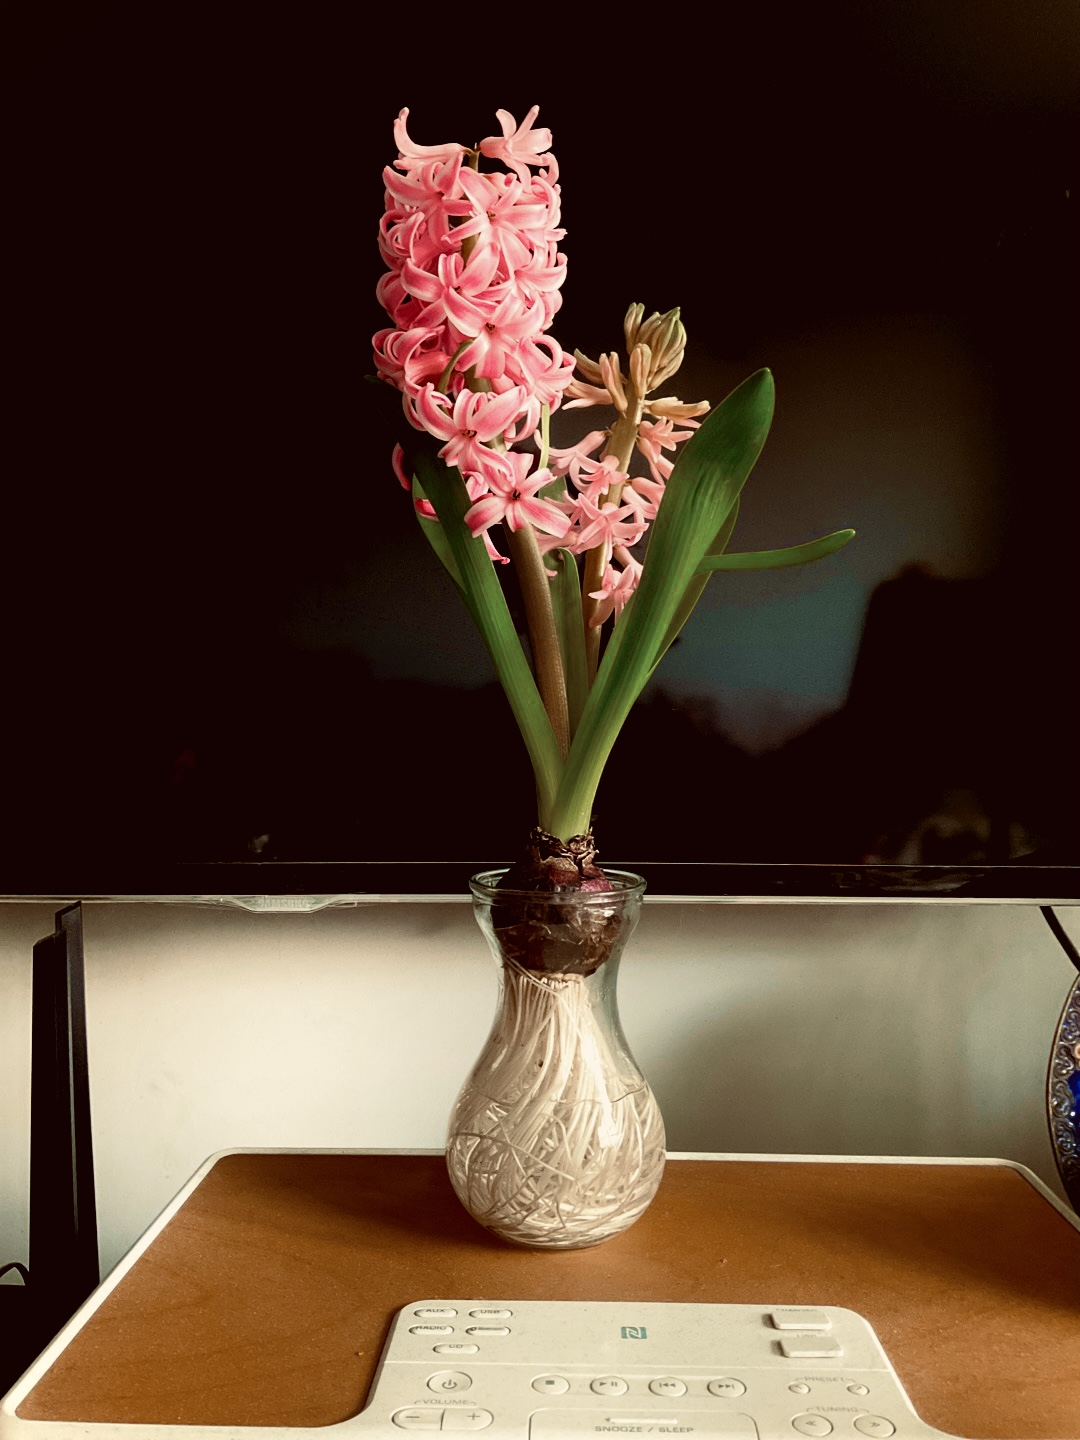
\includegraphics[width=5cm]{flower.jpeg}}\hfil}
\vfill\eject


%%% 2023年12月20日 星期三 12时43分48秒 CST
%%% author: Shao-Dan Lee 李小丹 字 殊恒

%%% cf. %%%%%%%%%%%%
%% texdoc: changelog, multicol, enumitem, cute
%% https://www.overleaf.com/learn/latex/Multiple_columns
%% https://tex.stackexchange.com/questions/10684/vertical-space-in-lists
%% https://tex.stackexchange.com/questions/282418/onecolumn-titlepage-twocolumn-rest-of-document
%% https://tex.stackexchange.com/questions/275264/switch-from-single-to-double-column-in-the-same-page

\pagemark{Changelog}{}
{%
\scriptsize
\columnseprule=0.5pt
\begin{multicols*}{2}[\section*{Changelog}]
%\begin{center}
%{\small\itemsep=1pt\parskip=1pt
\setlist{labelindent=5pt,noitemsep,nosep}
%\setlist{noitemsep}
%\setlist{nosep}
\begin{changelog}[author=李小丹, section=false]

\begin{version}[v=3.6-$\beta$(3.1415), date=2024-04-24]
	\added
		\item 在那遥远的地方
%	\fixed
%	\changed
%	\deprecated
%	\removed
%	\security
\end{version}
\begin{version}[v=3.5-$\beta$(3.1415), date=2024-04-03]
	\added
		\item 摇篮曲 -- 东北民歌, 捉泥鳅
%	\fixed
	\changed
		\item Using ``TeX Live 2024''
%	\deprecated
%	\removed
%	\security
\end{version}
\begin{version}[v=3.4-$\beta$(3.1415), date=2024-02-27]
	\added
		\item 曲谱: 广板
		\item 附录: 词汇缩写
		\item some midi files
	\fixed
		\item bug fixes
%	\changed
%	\deprecated
%	\removed
%	\security
\end{version}
\begin{version}[v=3.3-$\beta$(3.1415), date=2024-02-07]
	\added
		\item 红沙拉帆, 天国精灵舞曲, 萨拉班德舞曲
		\item some midi files
	\fixed
		\item bug fixes
	\changed
		\item BarNumber
%	\deprecated
%	\removed
%	\security
\end{version}
\begin{version}[v=3.2-$\beta$(3.1415), date=2024-01-04]
	\added
		\item 花儿与少年, 小天鹅舞曲, 苏武牧羊, 铃儿响叮当, 天鹅
		\item some midi files
	\fixed
		\item bug fixes
%	\deprecated
	\changed
		\item 前言
%	\removed
%	\security
\end{version}
\begin{version}[v=3.1-$\beta$(3.1415), date=2023-12-28]
	\added
		\item 步步高,乡间小路,铁血丹心,金蛇狂舞
		\item some midi files
%	\fixed
%	\deprecated
%	\changed
%	\removed
%	\security
\end{version}
\begin{version}[v=3.0-$\beta$(3.1415), date=2023-12-22]
	\added
		\item changlog page
		\item multicol: two columns pages
		\item enumitem, multicol, and changlog package
	\fixed
		\item page head marks of page "附录"
	\changed
		\item replace itemize, description by enumitem package
		\item enumitem: remove vertical space in lists
		\item enumitem: set labelindent in lists
		\item font size changlog
		\item book edition
		\item lilypond version
\end{version}
\begin{version}[v=2.9-$\beta$(3.141), date=2023-04-28]
	\added
		\item Scores
		\item midi files
		\item Music theory
	\fixed
		\item Bug fixes
\end{version}
\begin{version}[v=2.8-$\beta$(3.141), date=2023-04-24]
	\added
		\item Scores
		\item midi files
		\item Music theory
	\fixed
		\item Bug fixes
\end{version}
\begin{version}[v=2.7-$\beta$(3.141), date=2023-04-22]
	\added
		\item Scores
		\item midi files
		\item Music theory
	\fixed
		\item Bug fixes
\end{version}
\begin{version}[v=2.6-$\beta$(3.141), date=2023-04-15]
	\added
		\item Scores
		\item midi files
		\item Music theory
	\fixed
		\item Bug fixes
\end{version}
\begin{version}[v=2.5-$\beta$(3.141), date=2023-04-08]
	\added
		\item Scores
		\item Music theory
	\fixed
		\item Bug fixes
\end{version}
\begin{version}[v=2.4-$\beta$(3.141), date=2023-04-02]
	\added
		\item Scores
		\item Music theory
	\fixed
		\item Bug fixes
\end{version}
\begin{version}[v=2.3-$\beta$(3.141), date=2023-03-25]
	\added
		\item Scores
		\item Music theory
	\fixed
		\item Bug fixes
\end{version}
\begin{version}[v=2.2-$\beta$(3.141), date=2023-03-18]
	\added
		\item Scores
		\item Music theory
	\fixed
		\item Bug fixes
\end{version}
\begin{version}[v=2.1-$\beta$(3.141), date=2023-03-11]
	\added
		\item Scores
		\item Music theory
	\fixed
		\item Bug fixes
\end{version}
\begin{version}[v=2.0-$\beta$(3.141), date=2023-03-04, remark="Upload github"]
	\added
		\item Scores
		\item Music theory
	\fixed
		\item Bug fixes
\end{version}
\begin{version}[v=1.5-$\beta$(3.14), date=2023-02-21]
	\added
		\item Scores
		\item Appendix(Music theory)
	\fixed
		\item Bug fixes
%	\deprecated
%	\changed
%	\removed
%	\security
\end{version}
\shortversion{v=1.0-$\beta$(3.14),
	date=2023-01-30,
	changes=Initial beta\footnote{v2.9版本之前的changelog都是后补的,
		我早就忘记具体增改了什么,因此是不准确的。}}

\end{changelog}
%\end{center}
\end{multicols*}
\pagebreak[4]
}%


\ifodd\count0 \makeemptypage1\fi

\emptypage
\picbackground{harmonicaII.jpeg}{0.2}
\leavevmode\vfill
\ccby\hfill

\end{document}
